\documentclass{WileyMSP-template}

\usepackage{amsmath}
\usepackage{amssymb}


\begin{document}


\pagestyle{fancy}
%\rhead{\includegraphics[width=2.5cm]{vch-logo.png}}


\title{Influence of Illumination Spectrum on Dissociation Kinetics of Iron-boron Pairs in Silicon}

\maketitle



% Author: Please give full first and last names for authors and include * after the name of all corresponding authors

\author{Oleg Olikh*}
\author{Oleksandr Datsenko}
\author{Serhiy Kondratenko}

% Dedication

\dedication{}






% Affiliations: Please provide adacemic titles (Prof. or Dr.) for all authors where applicable, and include an institutional email address for all corresponding authors
\begin{affiliations}
Prof. O. Olikh, Dr. O. Datsenko, Prof. S. Kondratenko\\
Taras Shevchenko National University of Kyiv, 64/13, Volodymyrska Street, 01601, Kyiv, Ukraine\\
Email Address: olegolikh@knu.ua

%A. N. O. Author\\
%Address

\end{affiliations}


% Keywords: Please provide a minimum of three and a maximum of seven keywords, separated by commas

\keywords{silicon, iron-boron pairs, light-induced dissociation, wavelength impact, dissociation rate}



% Abstract should be written in the present tense and impersonal style (i.e., avoid we), and be at most 200 words long
\begin{abstract}

Photo-dissociation kinetics of iron–boron (FeB) pairs
in boron-doped Czochralski silicon was studied experimentally using different light sources.
It was shown that the FeB dissociation rate depends not only on integrated light intensity
and overall carrier generation rate, but also on spectral composition of illumination.
The value of the material constant of dissociation $K$ varies and has been determined to be within $(1.5-3.8)\times10^{-15}$~s.
The investigation has revealed an increase in the dissociation rate with increase in photon energy.
The results indicate that recombination-enhanced defect reaction is the primary factor in the second stage of pair dissociation.

\end{abstract}


% Text: Please use section headings and subheadings as specified below. For communications, all section headings apart from Experimental Section should be removed
% Please make the first reference to a display item bold: \textbf{Figure 1}
% Do not abbreviate Figure, Equation, etc.; display items are always singular, i.e., Figure 1 and 2.
% Equations are always singular, i.e., Equation 1 and 2, and should be inserted using the {equation} environment, not as graphics
% Please do not use footnotes in the text, additional information can be added to the Reference list.


\section{Introduction}

Defects significantly impact semiconductor properties.
Although when minimizing device dimensions to nanometers, focus some shifts from extended to point defects,
physical properties still rely heavily on the presence and distribution of these irregularities.
Hence, many strategies for enhancing semiconductor structures, including radiation and temperature treatments or certain fabrication conditions, strive to decrease the defect concentration or neutralize its effects \cite{Cai2023,Vobecky2021,Frascaroli2021}.
For instance, in the case of photovoltaic devices, we must understand and optimize the carrier properties related to defects and impurities  \cite{Cai2023}.
Such controlled alteration methods of the defect subsystem have been generalized under the term ``defect engineering'' and are extremely important from a practical standpoint.

Successful defect engineering hinges on an in-depth understanding of defect properties.
Key factors are defect formation energy, transition energy levels, self-compensating effects, nonradiative recombination caused by defects,
and the mechanism of reconstruction and diffusion  \cite{Cai2023}.
Considering the extraordinary diversity of possible intrinsic and impurity defects, information on them is incomplete,
even for silicon, which is the most studied semiconductor.
Nevertheless, it must be noted that considerable data have been amassed on silicon, resulting in a solid understanding of certain defects \cite{Juhl2018}.

For instance, iron impurity and iron-boron pairs are such defects that they are common, detrimental, and often unavoidable contaminants in photovoltaic silicon \cite{Frascaroli2021,Sun2021}.
Specifically, iron atoms are known to be at the interstitial sites, and Fe$_i^+$ are highly efficient recombination centers \cite{WeberFe}.
In p-type Si at room temperature, iron atoms are almost predominantly bound into complexes with dopants (B, Ga, Al, In).
This defect demonstrates bistable behavior: the stable state is defined by the configuration in which Fe occupies
the first nearest tetrahedral interstitial site closest to the substituent atom,
whereas, in the metastable configuration, Fe is at the second $T_d$ interstitial site \cite{FeB:PhysRevB49}.
The energy levels associated with iron and its complexes, as well as the respective carrier capture cross-sections, are well established \cite{Juhl2018,ROUGIEUX2018}.
Among the acceptor-iron pairs, the complex FeB is the most thoroughly investigated,
primarily due to the widespread use of Si:B in fabricating various devices, such as solar cells.
However, it is worth mentioning that gallium is gaining more and more attention as an acceptor dopant whose incorporation,
for instance, can help mitigate light and elevated temperature-induced degradation \cite{Ning2022}.

The dynamics of FeB pairs are also examined.
It's established that FeB pairs can be dissociated through illumination, minority carrier injection, and thermal treatment at 200~$^\circ$C \cite{FeBAssJAP2014}.
In the context of illumination, the dissociation rate $R_d$ is influenced by the overall carrier generation rate $G$ \cite{FeBLight2,FeBAssJAP2014,FeBKin2019,FeMethod2012}:
\begin{equation}
\label{eqRd}
R_d=K\left(\frac{G}{N_\mathrm{FeB}}\right)^2\,,
\end{equation}
where
$N_\mathrm{FeB}$ is the pair concentration,
$K$ is the constant of the material.
It is necessary for the illumination power to exceed 0.1~W~cm$^{-2}$ to achieve almost complete dissociation of the FeB pairs \cite{Macdonald2004}.
The dissociation process of FeB pairs by electron capture unfolds in two stages \cite{KIMERLINGFeB,FeBAssJAP2014}:
the initial one involves the neutralization of Fe and the elimination of the Coulomb attraction between the pair components.
The mechanism of the second stage is contentious; it may involve either the recharge of the iron ion or the recombination-enhanced defect reaction
(REDR) triggered by electron-hole recombination.


It should be noted that despite the extensive data on the properties of iron-related defects in silicon, intensive research continues.
In particular, efforts focus on analyzing the impact of high-intensive  illumination \cite{FeBStrongIll}
or dopant compensation \cite{Zhu2015},
alongside clarifying the second-stage mechanism of dissociation \cite{Sun2021}
or reassessing recombination parameters \cite{Le2024}.

This study aims to investigate the effect of the light spectrum on the dissociation kinetics of FeB pairs in silicon.
While pair dissociation is typically carried out using a halogen lamp \cite{FeBLight2,Sun2021}
or a 904 nm laser \cite{FeBStrongIll,FeBAssJAP2014,lauer2016}, there is limited understanding of how the light source influences this process.
By studying the impact of different illumination spectra on FeB dissociation,
we aim to provide valuable insights for defect engineering and the efficient transformation of detrimental impurity iron atoms into a highly mobile interstitial state
within the active region of a silicon device.
Besides, such information, in our opinion, can help make the right choice between existing options for the second stage of pair decay.

In \textbf{Figure~\ref{fig1}}, the main stages of the research are illustrated.
First step was the determination of the dissociation rate of FeB pairs under illumination with different integral intensities.
Three light sources from different manufacturers were used (box 1 on Figure~\ref{fig1}, further details are described in Section~\ref{SecExp}).
The kinetics of short-circuit current were used (boxes 2 and 3) to measure the number of interstitial iron atoms formed over fixed time under intense illumination (box~4).
The result is presented in Subsection~\ref{SecR}.
Second step and Subsection~\ref{SecG} deal with estimating the carrier generation rate using spectra of sample illumination (box~5) and considering the effects of light reflection,
absorption by free carriers, and effective absorption depths (box~6).
The results showed that light--induced dissociation efficiency increases with decreasing photon wavelength --- see Subsection~\ref{SecLast} and box~7.
Finally, we conclude this paper in Section~\ref{SecConsl} (box~8).

\begin{figure}
\centering
  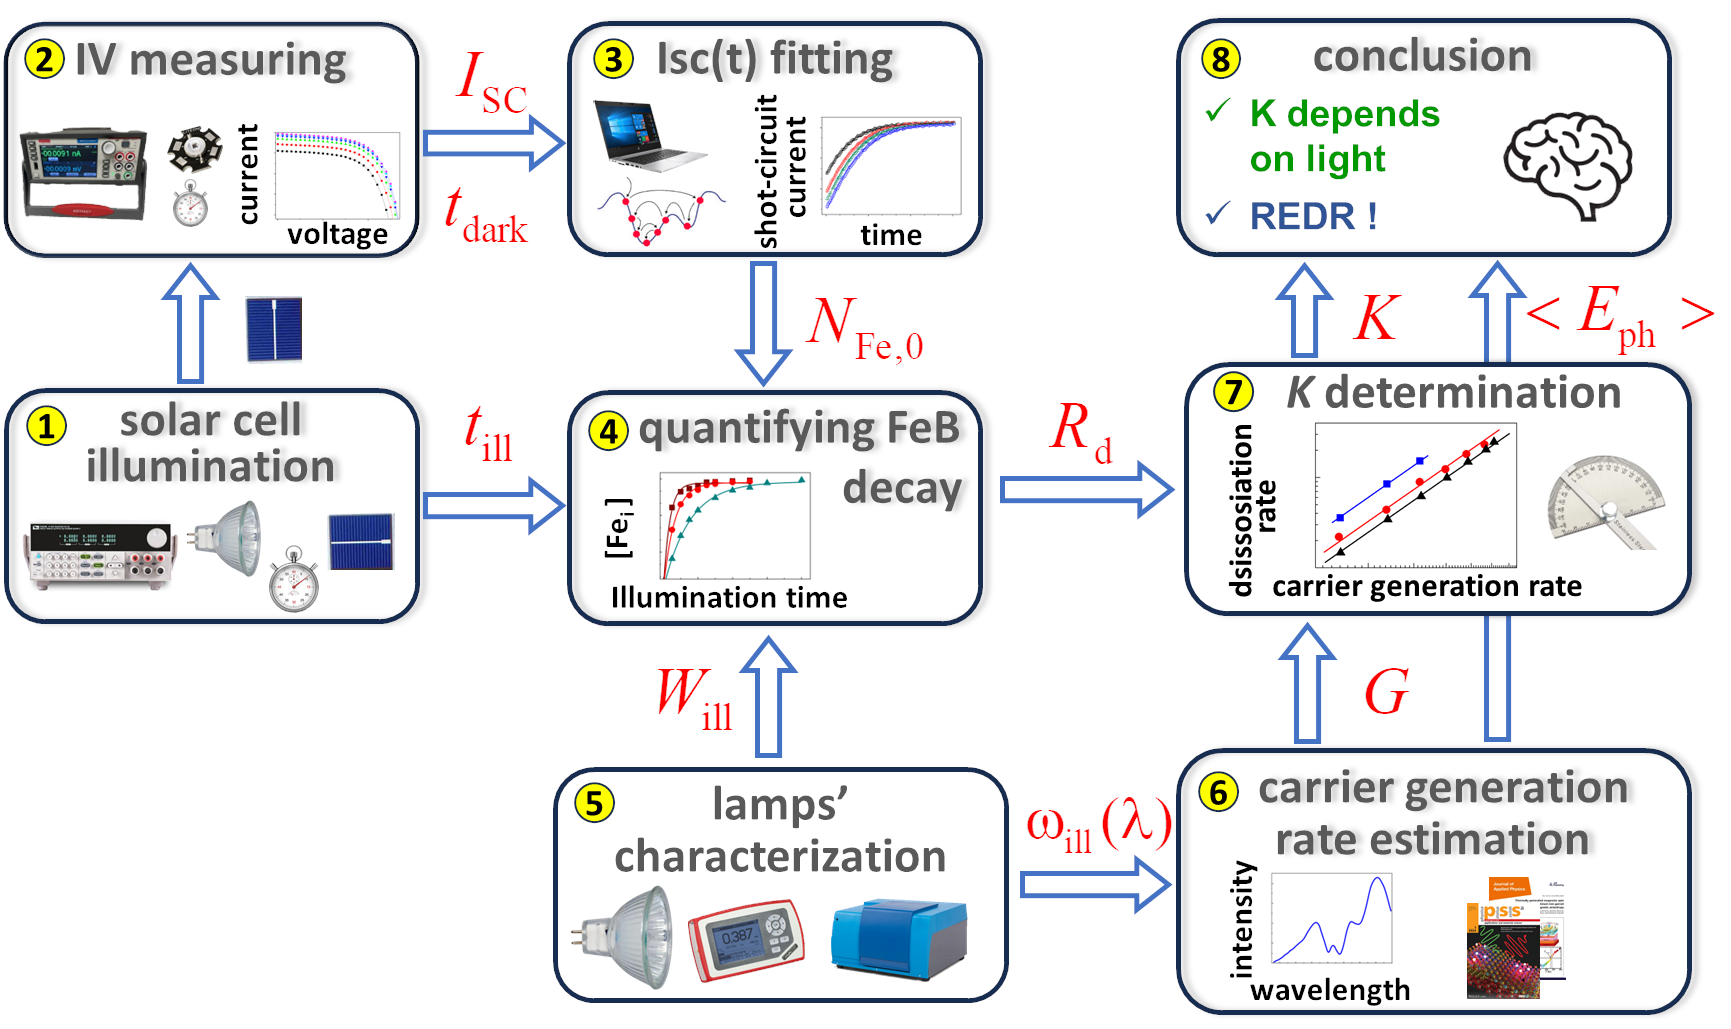
\includegraphics[width=0.7\linewidth]{Fig1.png}
  \caption{Investigation framework}
  \label{fig1}
\end{figure}


\section{Results and Discussion}

\subsection{Dissociation rate determination}\label{SecR}

The equilibrium between free Fe$_i$ and Fe$_i$B$_\mathrm{Si}$ is known to be determined by the following equations \cite{FeB:kinetic,Sun2021,FeBAssJAP2014}
\begin{equation}
\label{eqReac}
\mathrm{Fe}_i+\mathrm{B}_\mathrm{Si}  \overset{R_a}{\underset{R_d}{\rightleftharpoons{}}} \mathrm{FeB}\,,
\end{equation}
where
$R_a$ is the association rate.
As a result, the concentration of unpaired interstitial iron atoms $N_\mathrm{Fe_i}$ depending on illumination time $t_\mathrm{ill}$
during light-induced dissociation can be described as follows \cite{FeBLight2,FeBKin2019,Olikh2021JAP}
\begin{equation}
\label{eqNfeill}
N_\mathrm{Fe_i}(t_\mathrm{ill})=\left(N_\mathrm{Fe,eq}-N_\mathrm{Fe,tot}
\frac{R_d}{R_d+R_a}\right)\exp[-(R_d+R_a)t_\mathrm{ill}]+N_\mathrm{Fe,tot}\frac{R_d}{R_d+R_a}\,,
\end{equation}
where
$N_\mathrm{Fe,tot}$ is the total concentration of the impurity iron,
$N_\mathrm{Fe,eq}$ represents the concentration of unpaired interstitial iron atoms in the equilibrium state
(in darkness, $N_\mathrm{Fe,eq}=N_\mathrm{Fe_i}(t_\mathrm{ill}\leq0)$).
It is important to highlight that $N_\mathrm{Fe,eq}$ is significantly influenced
by temperature and the Fermi level location \cite{FeB:kinetic}.
Specifically, in the case of p-type Si with a hole concentration $p=1.36\times10^{15}$~cm$^{-3}$
(which corresponds to the structure under investigation),
at a temperature of $T=300$~K, $N_\mathrm{Fe,eq}$ is about 1 percent of $N_\mathrm{Fe,tot}$,
which is negligible for practical considerations.
However, when the temperature rises to 340~K, the proportion of $N_\mathrm{Fe,eq}$ increases to approximately 14.5\%.


After stopping the illumination, only the process of association occurs,
and the time dependence of Fe$_i$ concentration can be expressed as follows \cite{FeB:kinetic,MurphyJAP2011}:
\begin{equation}
\label{eqNFet}
N_\mathrm{Fe_i}(t_\mathrm{dark})=(N_\mathrm{Fe,0}-N_\mathrm{Fe,eq})\times
\exp(-R_a t_\mathrm{dark})+N_\mathrm{Fe,eq}\,,
\end{equation}
where $t_\mathrm{dark}$ is the time after stopping the intense illumination,
$N_\mathrm{Fe,0}$ is the concentration of interstitial iron atoms formed after illumination,
$N_\mathrm{Fe,0}=N_\mathrm{Fe_i}(t_\mathrm{dark}=0)=N_\mathrm{Fe_i}(t_\mathrm{ill})$.

The study examined the dependence of $N_\mathrm{Fe,0}$ in silicon solar cells on illumination time $t_\mathrm{ill}$
using different integral illumination intensities $W_\mathrm{ill}$ ($200-750$~mW) and light sources
(three halogen lamps labeled as Orion, Osram, and GE and described in detail in Section~\ref{SecExp}).
The experiments were conducted at a temperature of 340~K.
The values of $N_\mathrm{Fe,0}$ were  determined using a methodology \cite{Olikh2022:JMatSci,Olikh2021JAP}
based on fitting the kinetics of short-circuit current $I_{SC}$ under low-intensity monochromatic illumination.
Specifically, after intense illumination with a duration of $t_\mathrm{ill}$,
the current-voltage characteristic ($I$-$V$) of the solar cell was measured every 21 seconds over a time $t_\mathrm{dark}$ of about 3000 seconds.

\textbf{Figure~\ref{fig2}a} shows some typical $I$-$V$ curves.
A gradual increase in both the short--circuit current and the open--circuit voltage is observed after the cessation of illumination.
This indicates a decrease of the recombination activity of the defect subsystem,
which is a result of the transition of interstitial iron to the bound state with the acceptor.
Moreover, negligible changes in the $I$-$V$ curves at the end of the measurement interval denote that the selected interval of 50 minutes is sufficient for complete association.


\begin{figure}
\centering
  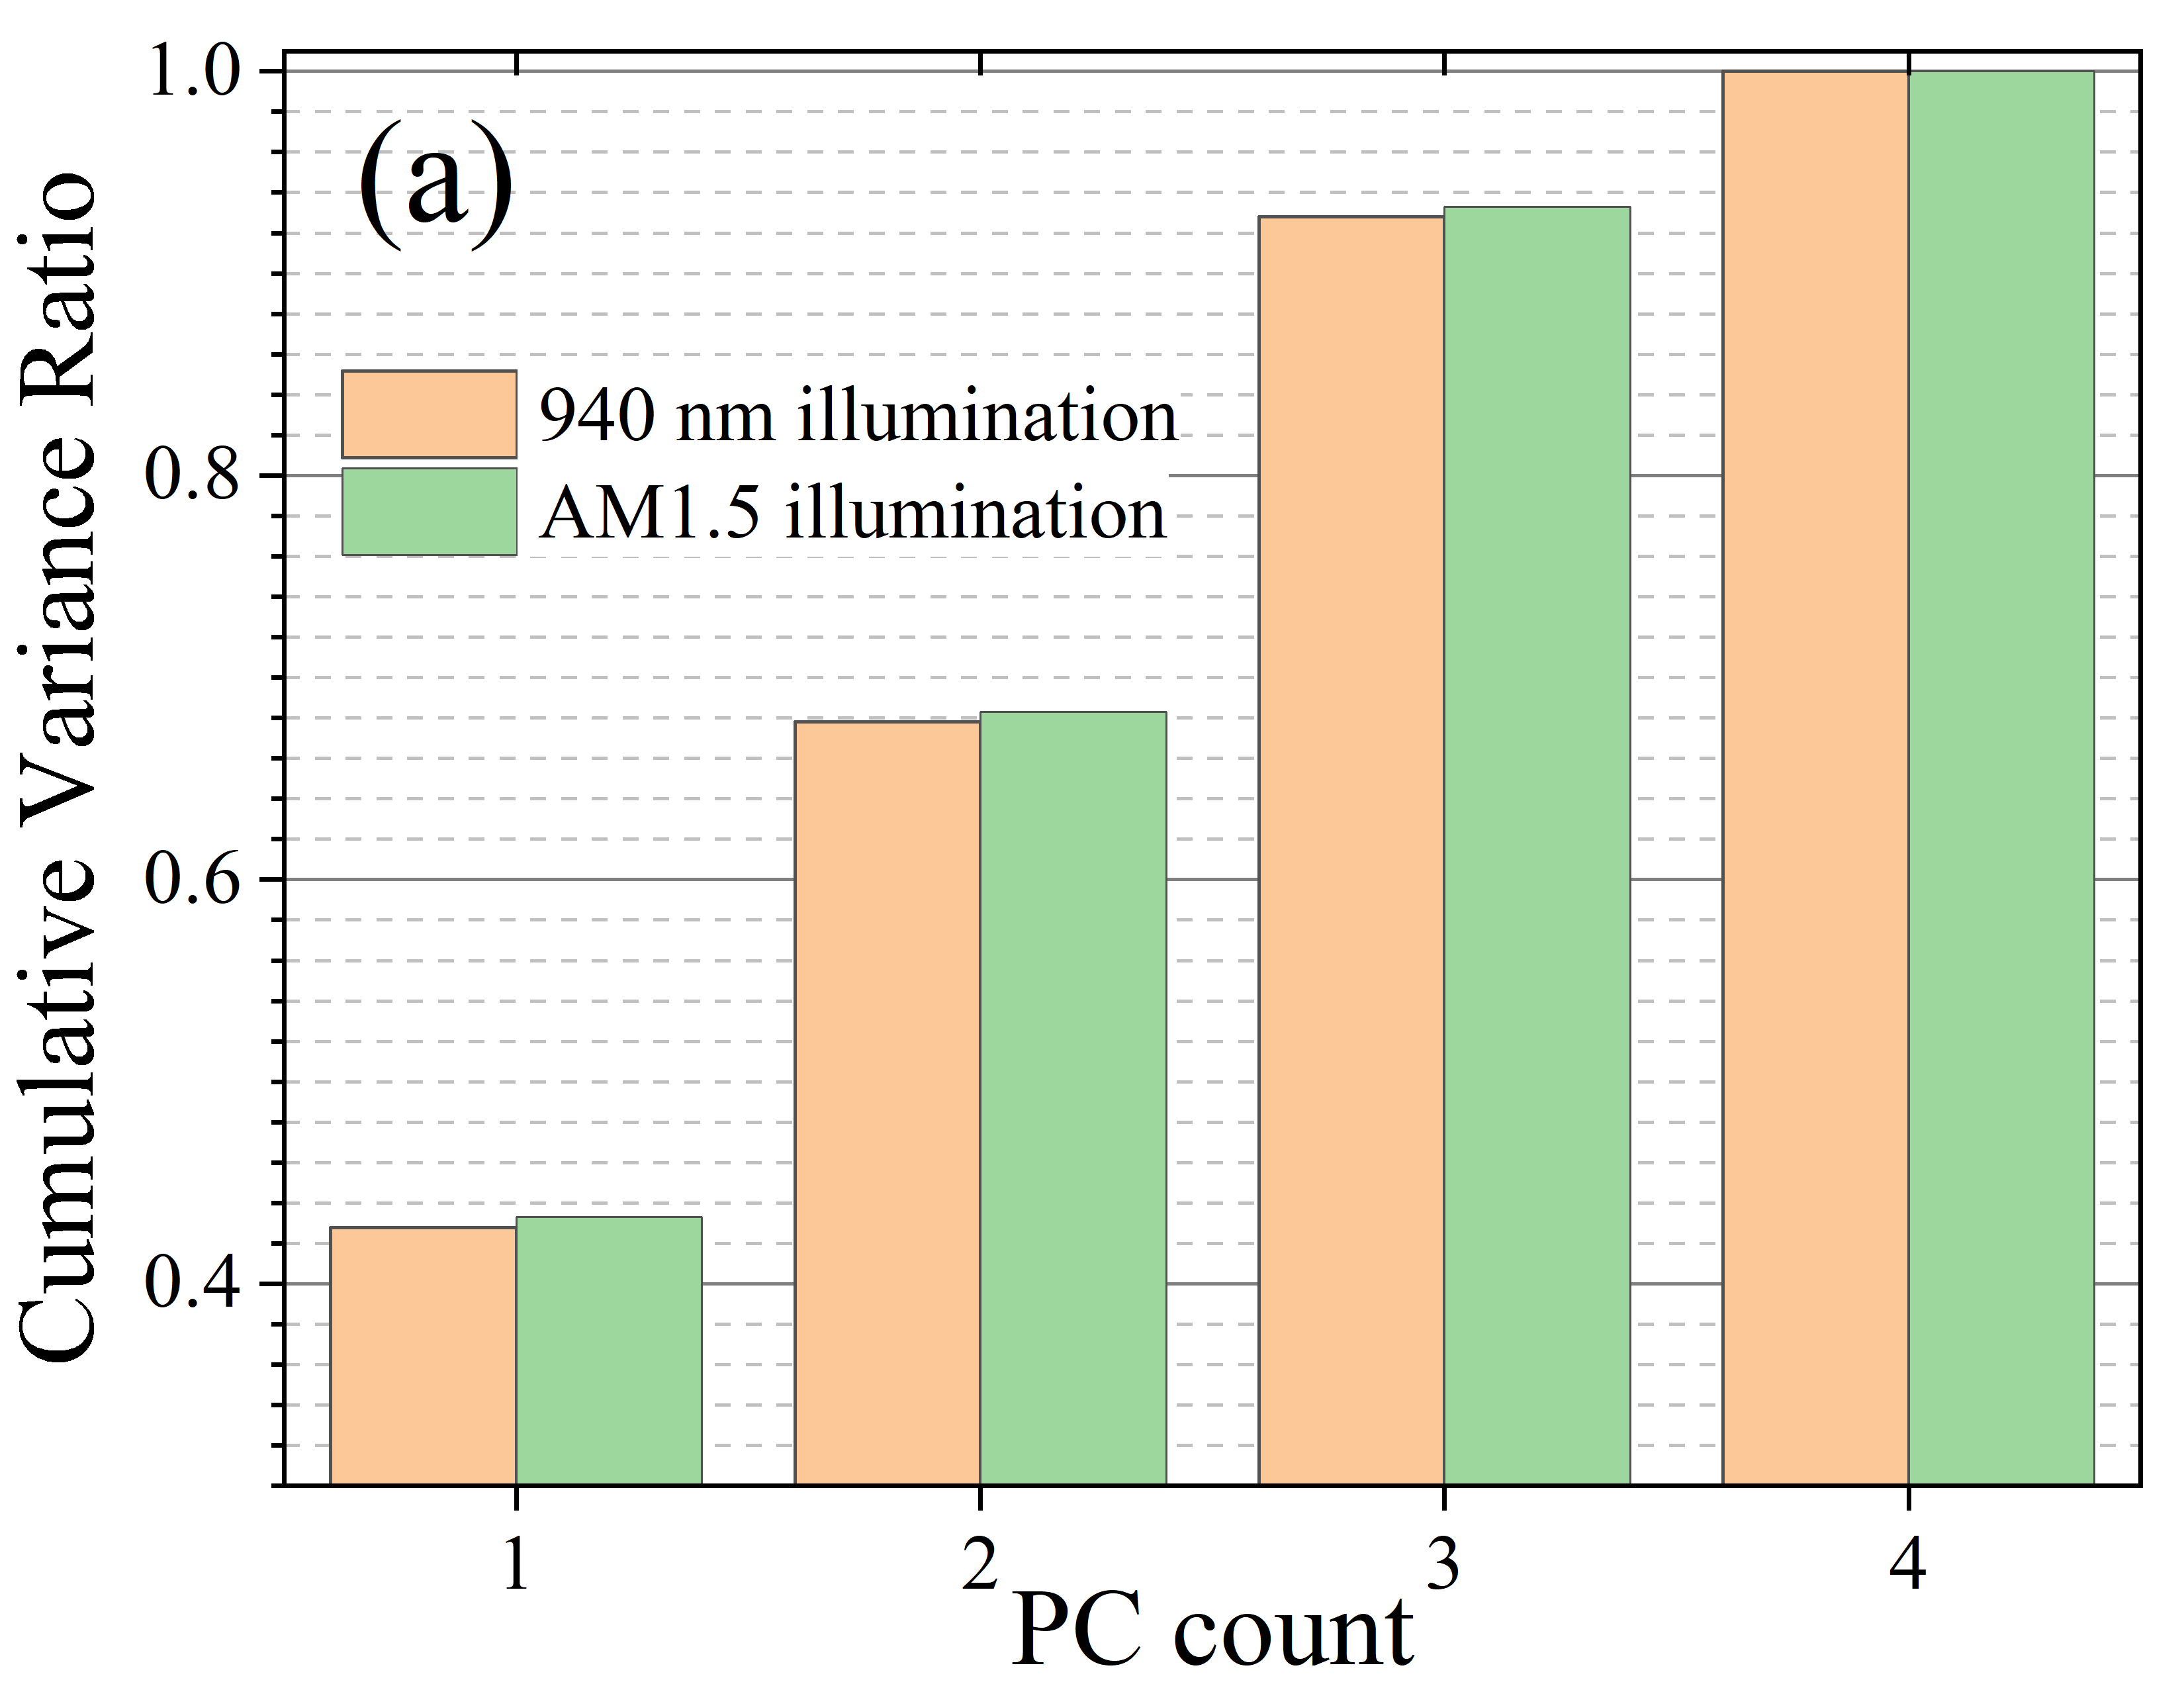
\includegraphics[width=0.4\linewidth]{Fig2a.png}
  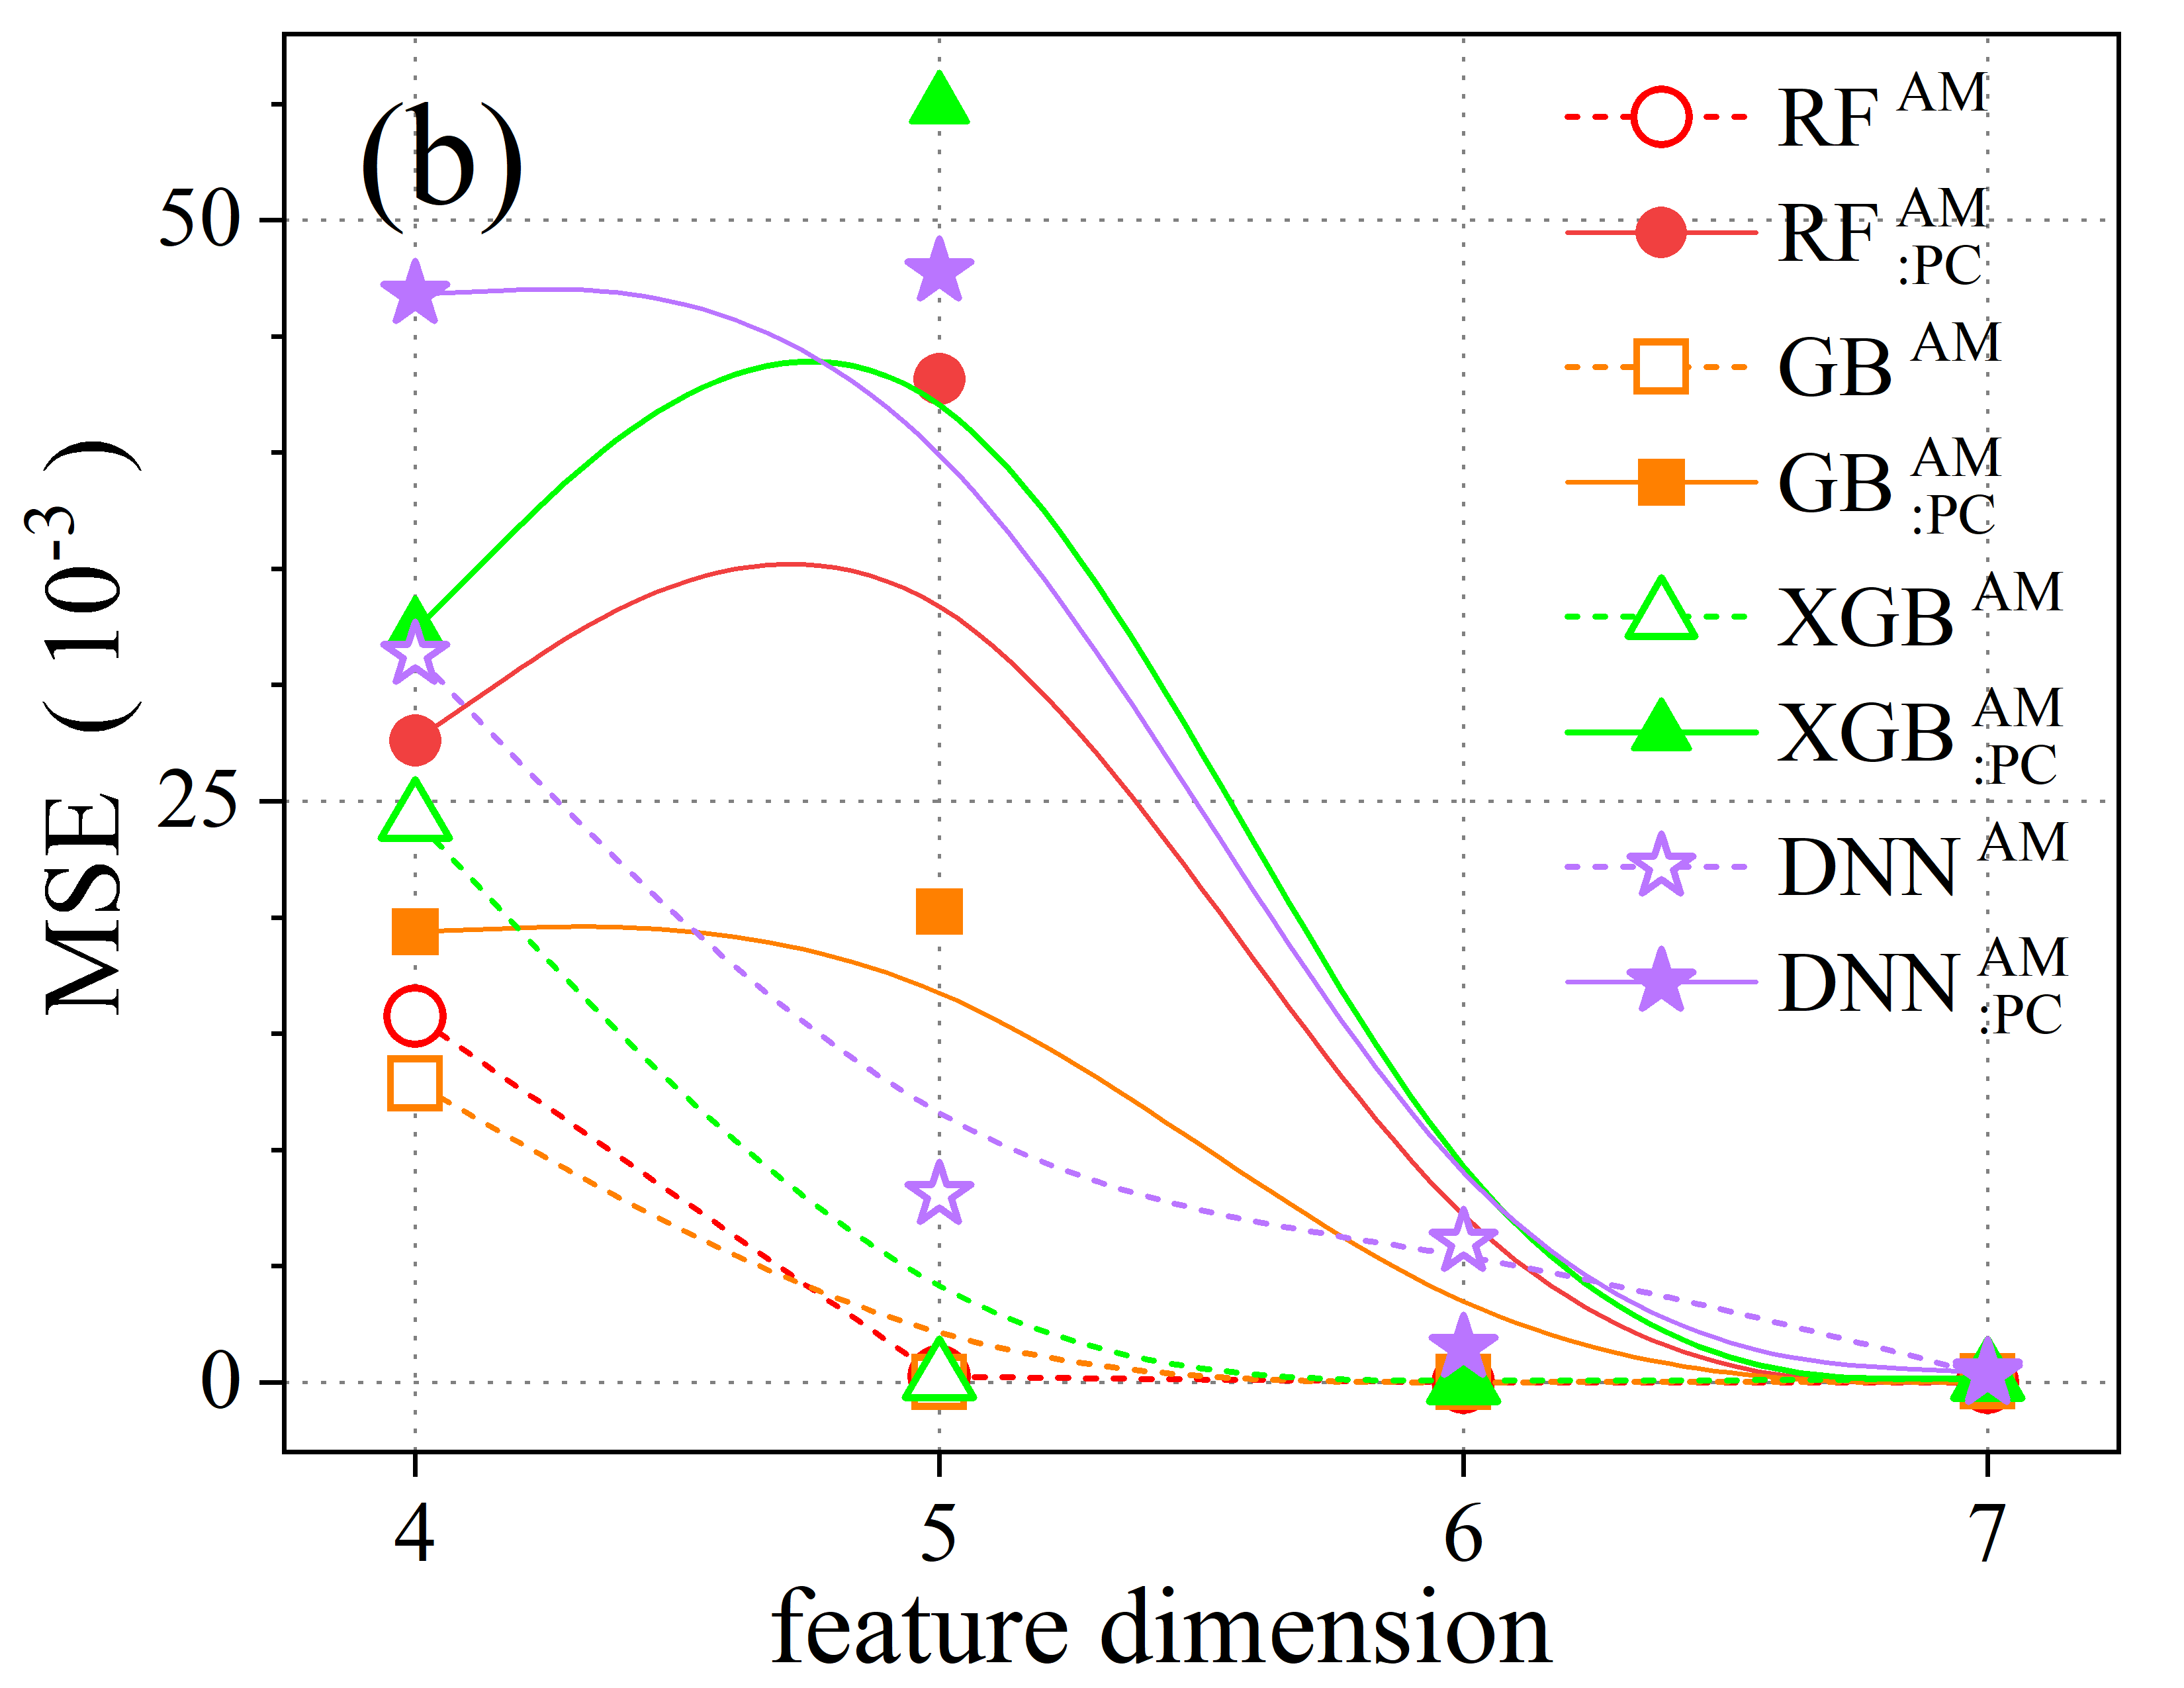
\includegraphics[width=0.4\linewidth]{Fig2b.png}
  \caption{Typical $I$-$V$ characteristics measured at $T=340$~K
  under low--intense LED illumination at 940~nm after delays following the exposure for 50~s to intense (400~mW) light (GE lamp) (a) and
  short circuit current vs the delay time after the illumination for 5~s of Osram lamp with various intensities (b).
  The marks are the experimental data, and the lines on (b) are the fitting curves according to \cite{Olikh2022:JMatSci,Olikh2021JAP}.
  }
  \label{fig2}
\end{figure}

\textbf{Figure~\ref{fig2}b} illustrates the dependencies $I_{SC}(t_\mathrm{dark})$ after the illumination with different intensities.
As shown previously \cite{Olikh2021JAP}, the magnitude of the change in $I_{SC}$ after the dark recovery period
inherently correlates with the concentration of Fe$_i$ formed due to the light--induced dissociation of FeB pairs.
The presented data evidence that the rise of $W_\mathrm{ill}$ leads to an increment in the dissociation efficiency.
Meanwhile, the recovery time remains insensitive to the illumination parameters, which is expected, as the former is determined by $R_a$ (see Equation~(\ref{eqNFet})).

It should be noted that apart from $N_\mathrm{Fe,0}$,
the fitting of short-circuit current \cite{Olikh2022:JMatSci,Olikh2021JAP} allows for the estimation of the migration energy of Fe$_i$, $E_m$,
and bulk lifetime $\tau_\mathrm{other}$ of minority carriers, which is related to recombination channels other than Fe-related defects and intrinsic recombination.
The obtained value $E_m=(0.650\pm0.005)$~eV coincides with that known from Refs. \cite{FeBKin2019,FeBAssSST2011,FeBkinAPL2008}.
This coincidence confirms that the investigated processes are indeed associated with rebuilding,
as Equation~(\ref{eqReac}) describes.
In turn, the value of $E_m$ allows for the estimation of the association rate \cite{FeBAssJAP2014,FeBKin2019,FeBAssSST2011}:
\begin{equation}
\label{eqTass}
R_a^{-1}=5.7\times10^5\,\frac{\mathrm{s}}{\mathrm{K}\;\mathrm{cm}^3}\times\frac{T}{p}\exp\left(\frac{E_m}{kT}\right)\,.
\end{equation}
Thus, in our case, $R_a=(1.68\pm0.03)\times10^{-3}$~s$^{-1}$.

As for the value of $\tau_\mathrm{other}$, it was found to exceed significantly the
lifetime associated with Shockley--Read--Hall (SRH) recombination on Fe--related defects.
The last one is about $2.2$~$\mu$s, whereas $\tau_\mathrm{other}$ equals $(20-300)$~$\mu$s for the samples of the same series.
Notably, according M\"{o}ller~\emph{et al.} \cite{FeBAssJAP2014},
such a condition is essential for accurately determining the constant $K$, which is included in Equation~(\ref{eqRd}).

The dependencies of the concentration of interstitial atoms on illumination time are shown in \textbf{Figure~\ref{fig3}}.
It is evident from the data that the pair dissociation rate is influenced significantly by the illumination intensity for all the used light sources.
Nonetheless, the pair dissociation rate is not determined by the $W_\mathrm{ill}$ value only.
As demonstrated in Figure~\ref{fig3}d, pair dissociation under the GE source is the fastest.
With Osram under otherwise identical conditions, the process is slower,
while illumination with Orion proves to be the least effective in terms of altering the state of FeB pairs.


\begin{figure}
\centering
  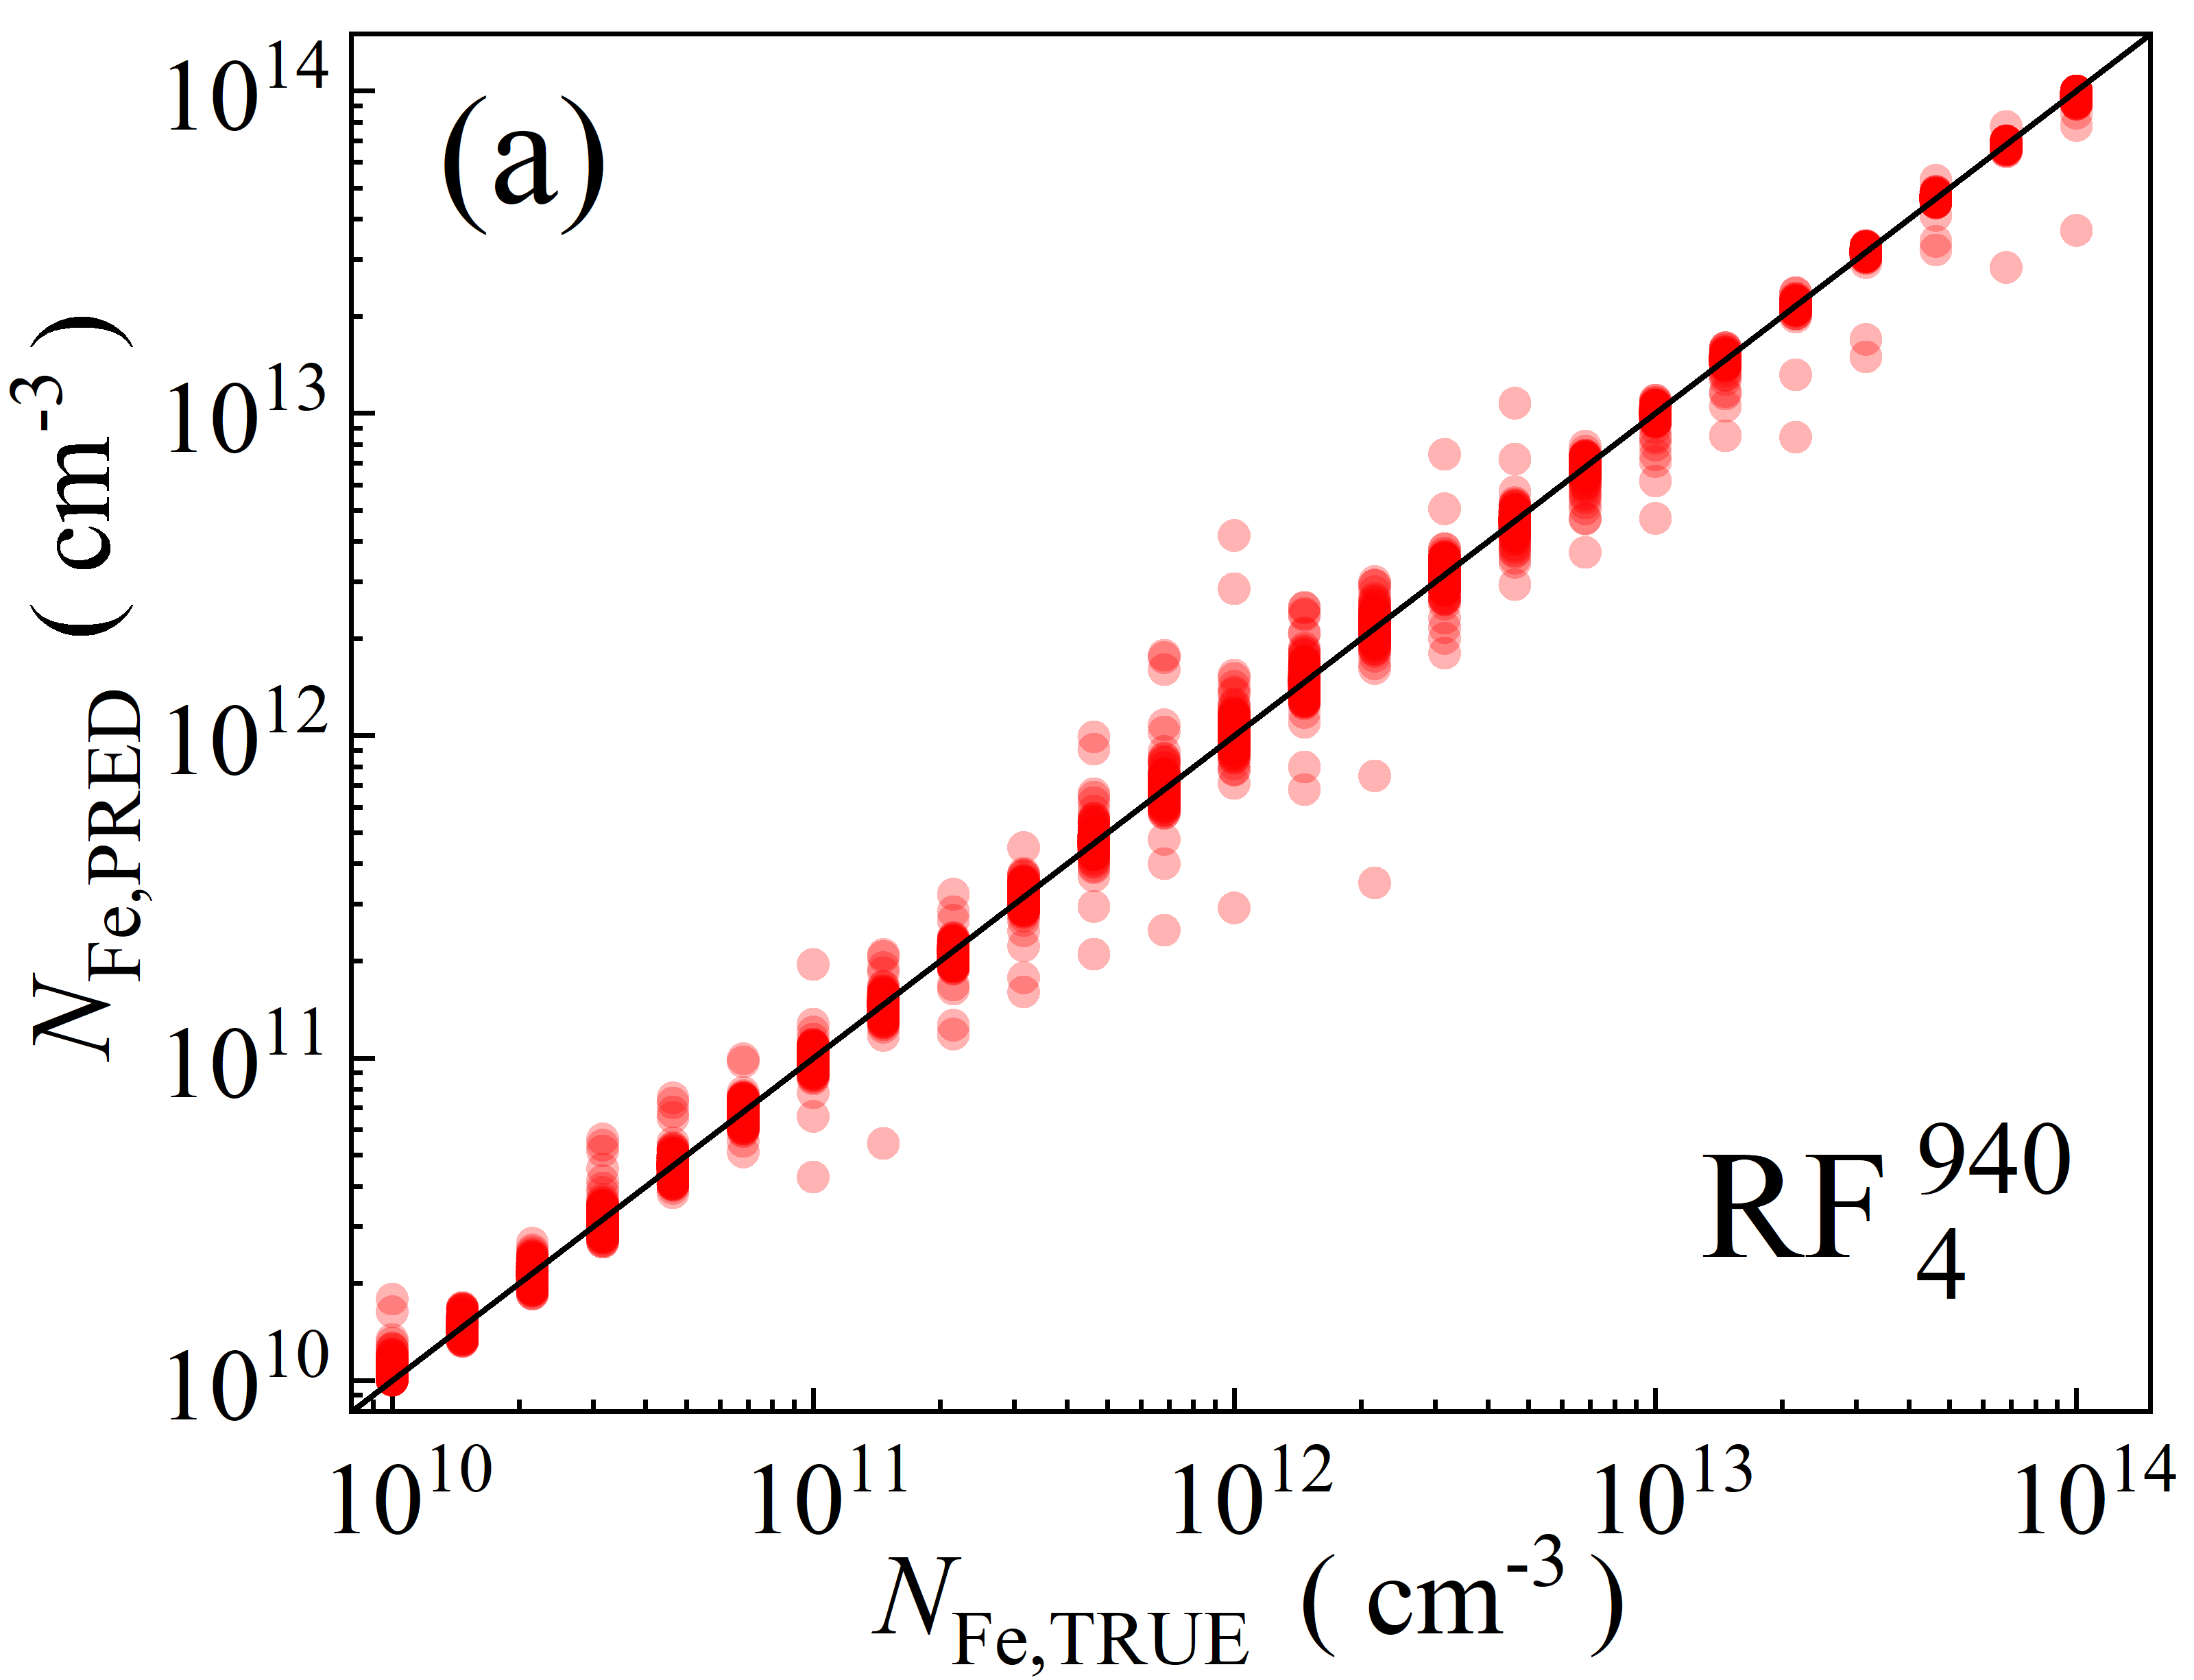
\includegraphics[width=0.4\linewidth]{Fig3a.png}
  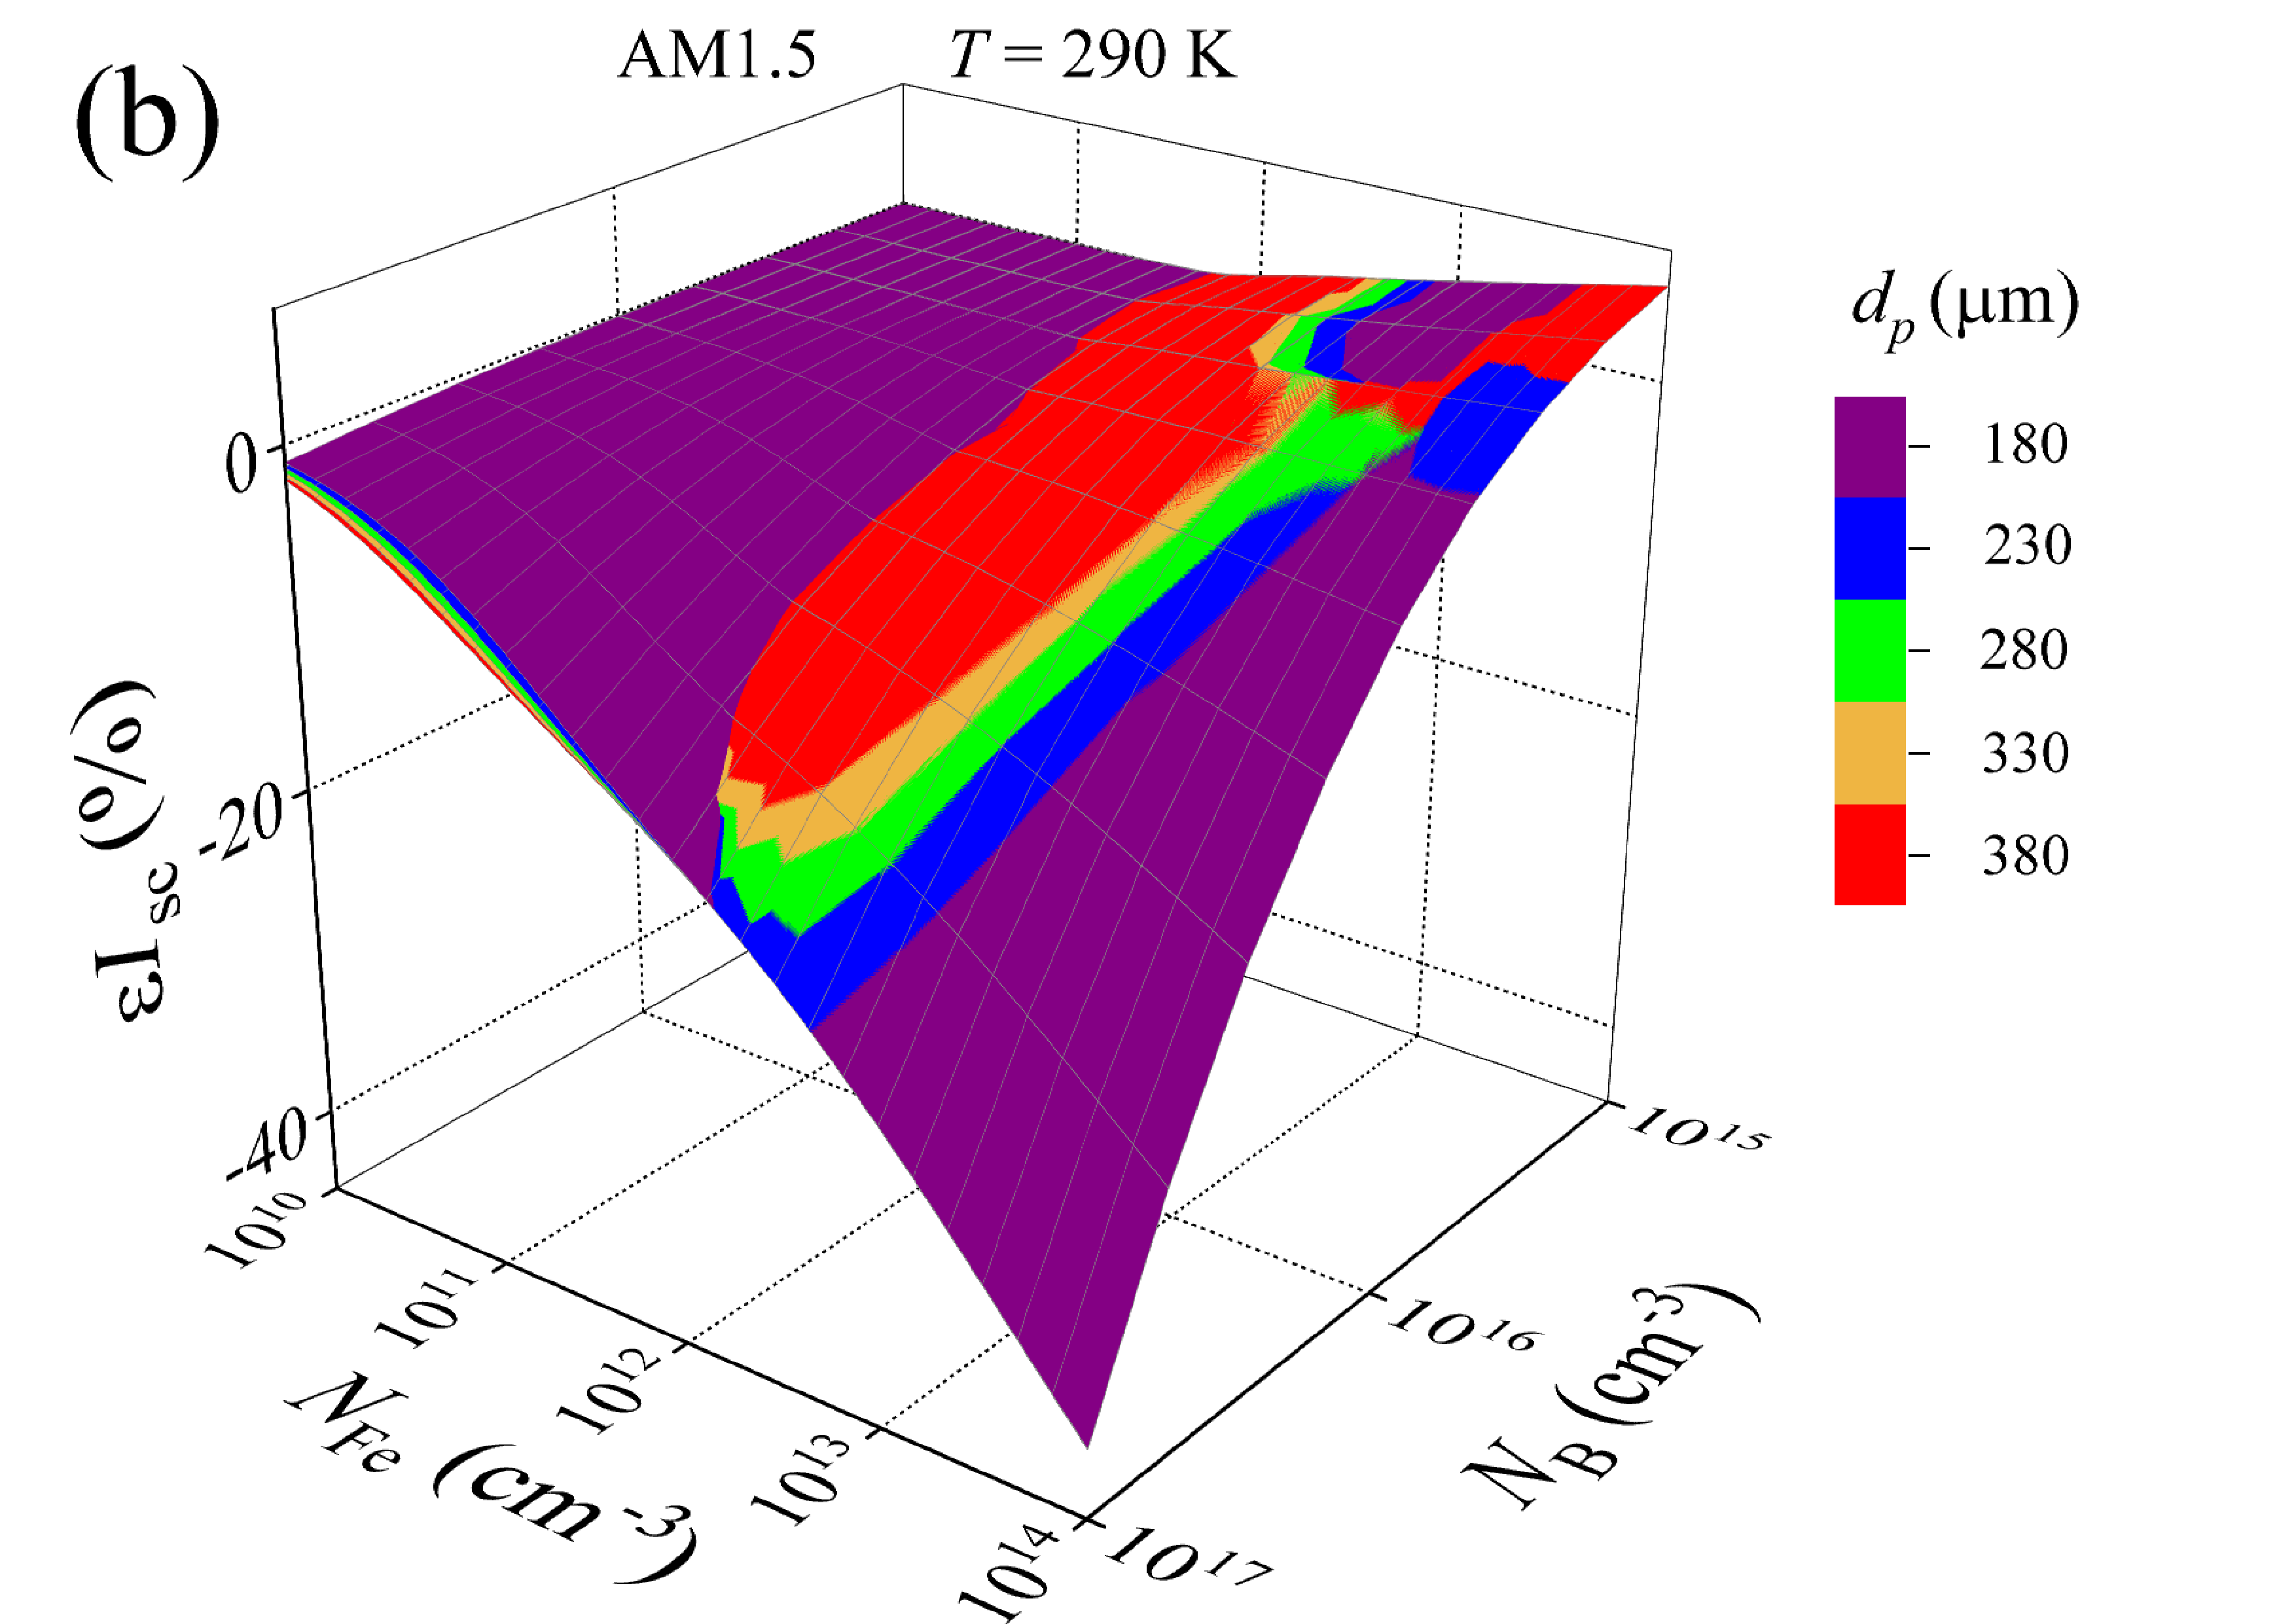
\includegraphics[width=0.4\linewidth]{Fig3b.png}
  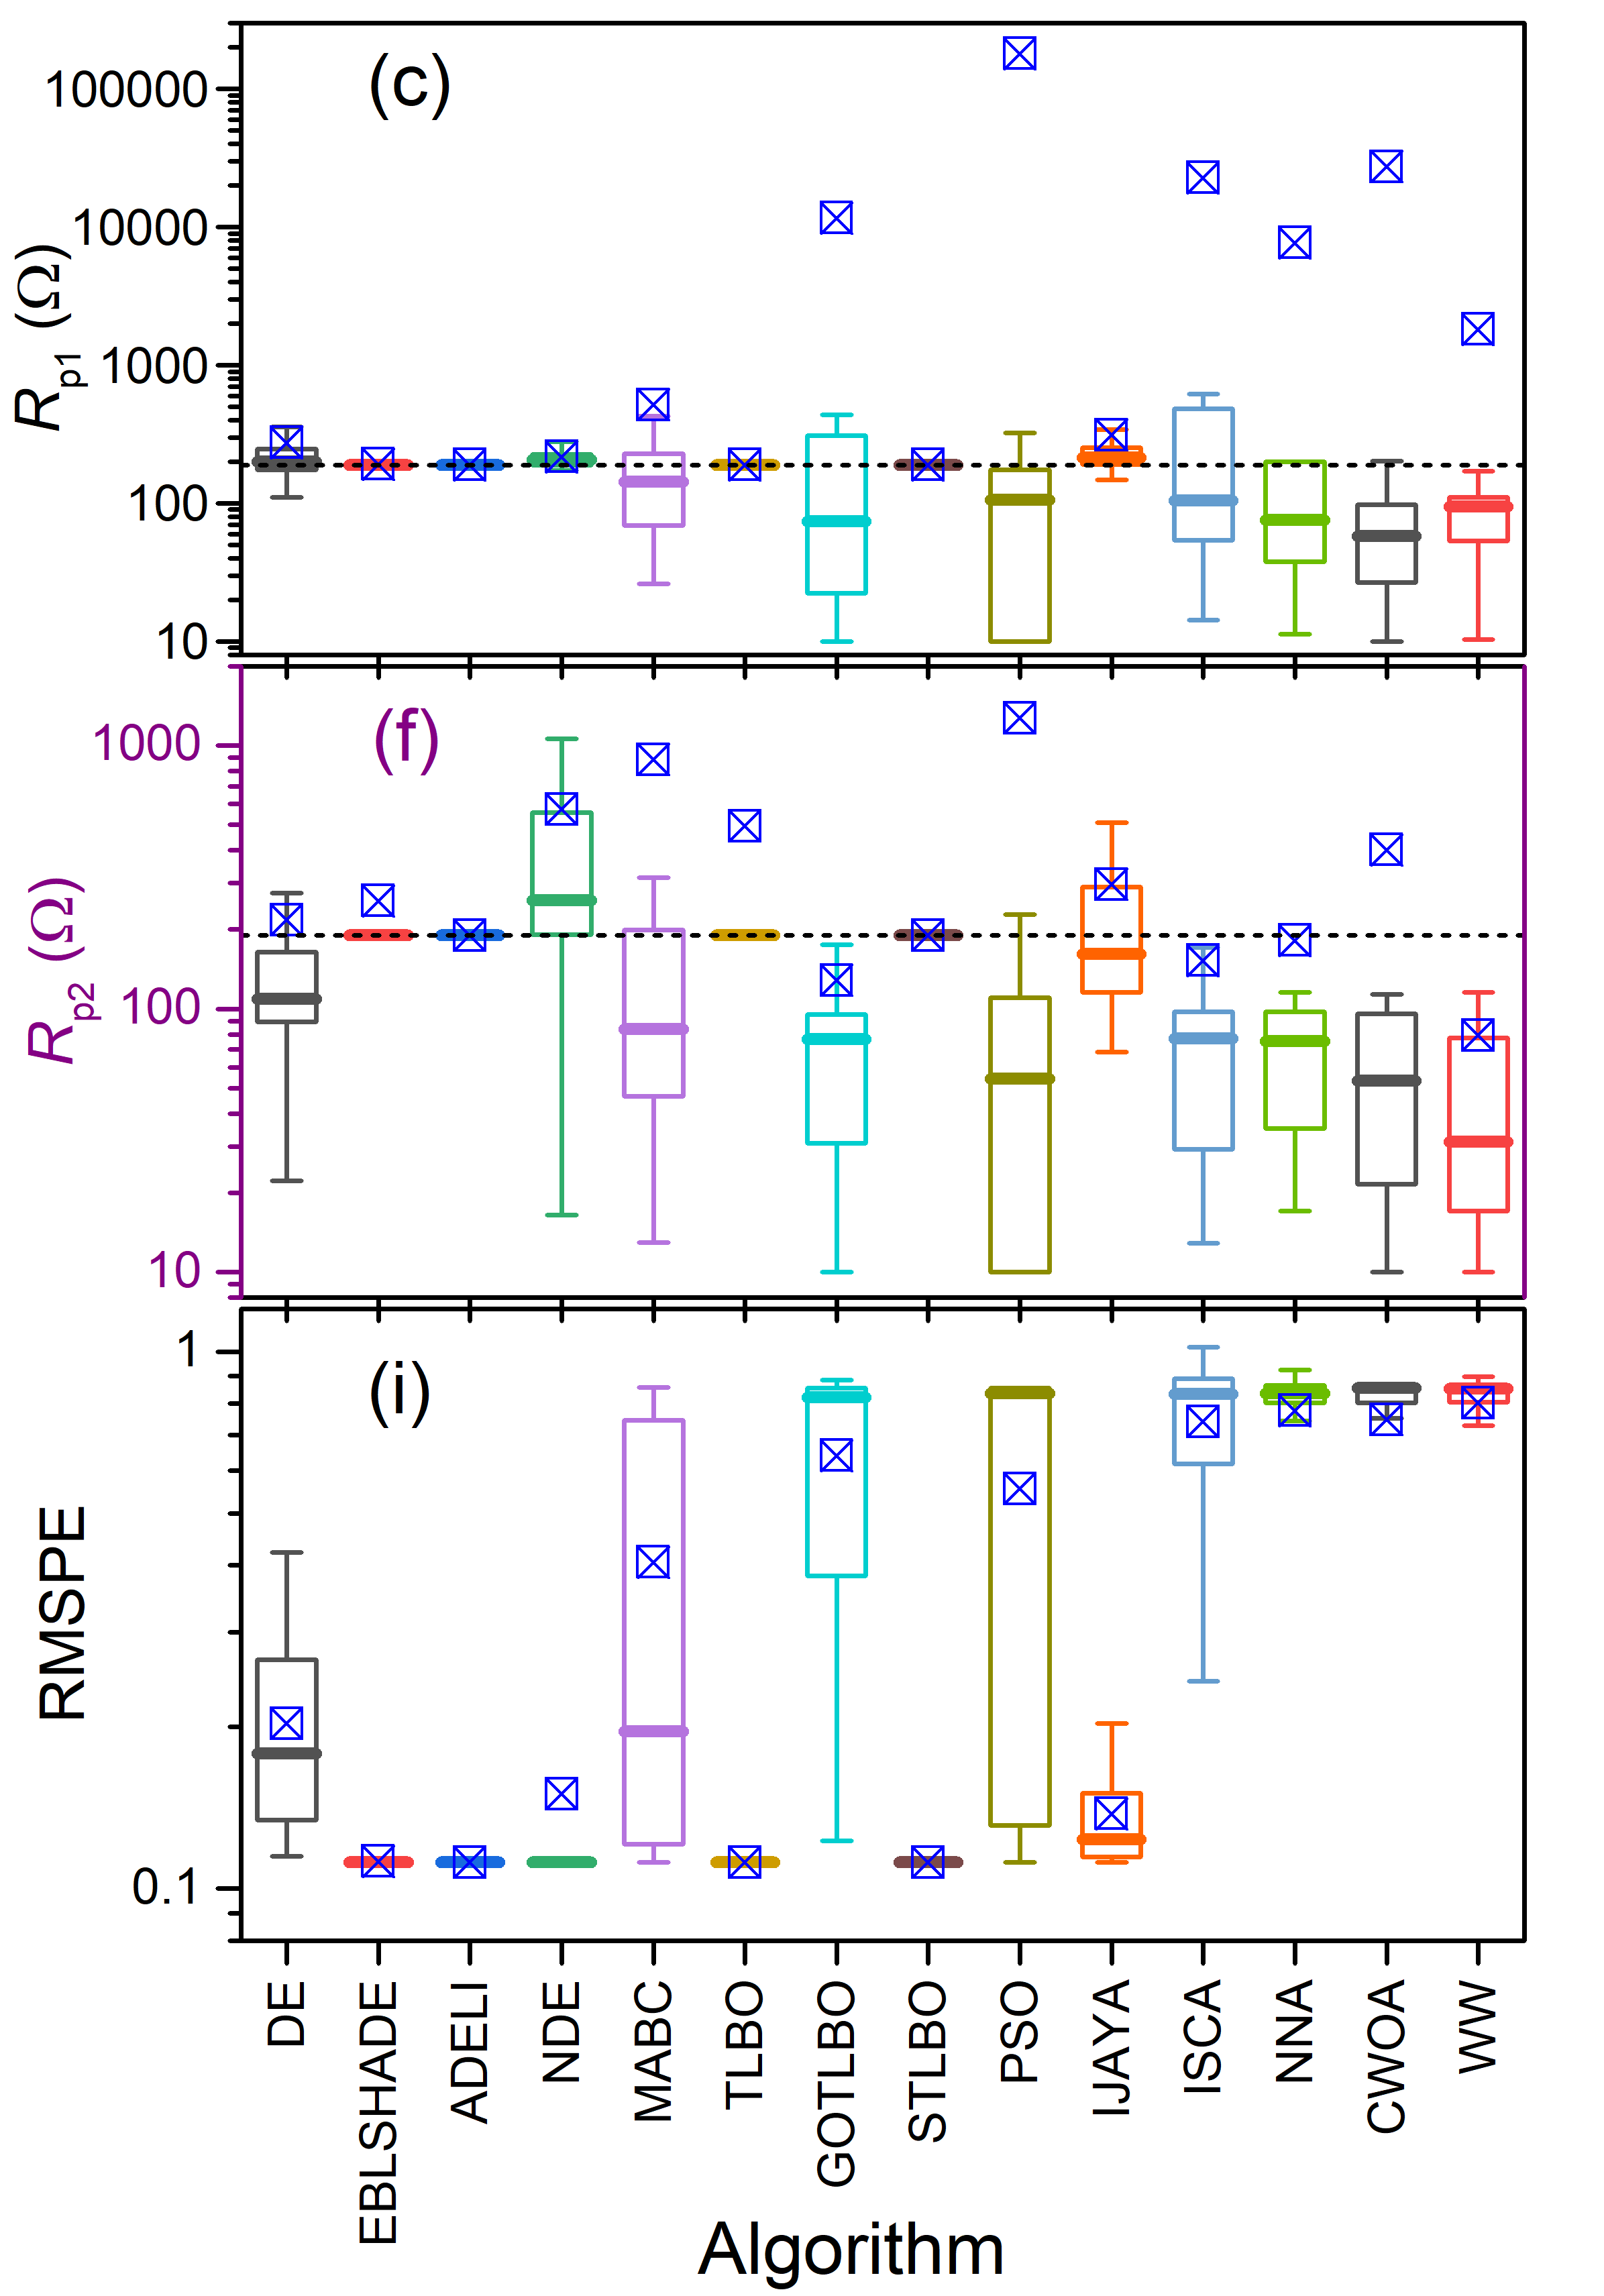
\includegraphics[width=0.4\linewidth]{Fig3c.png}
  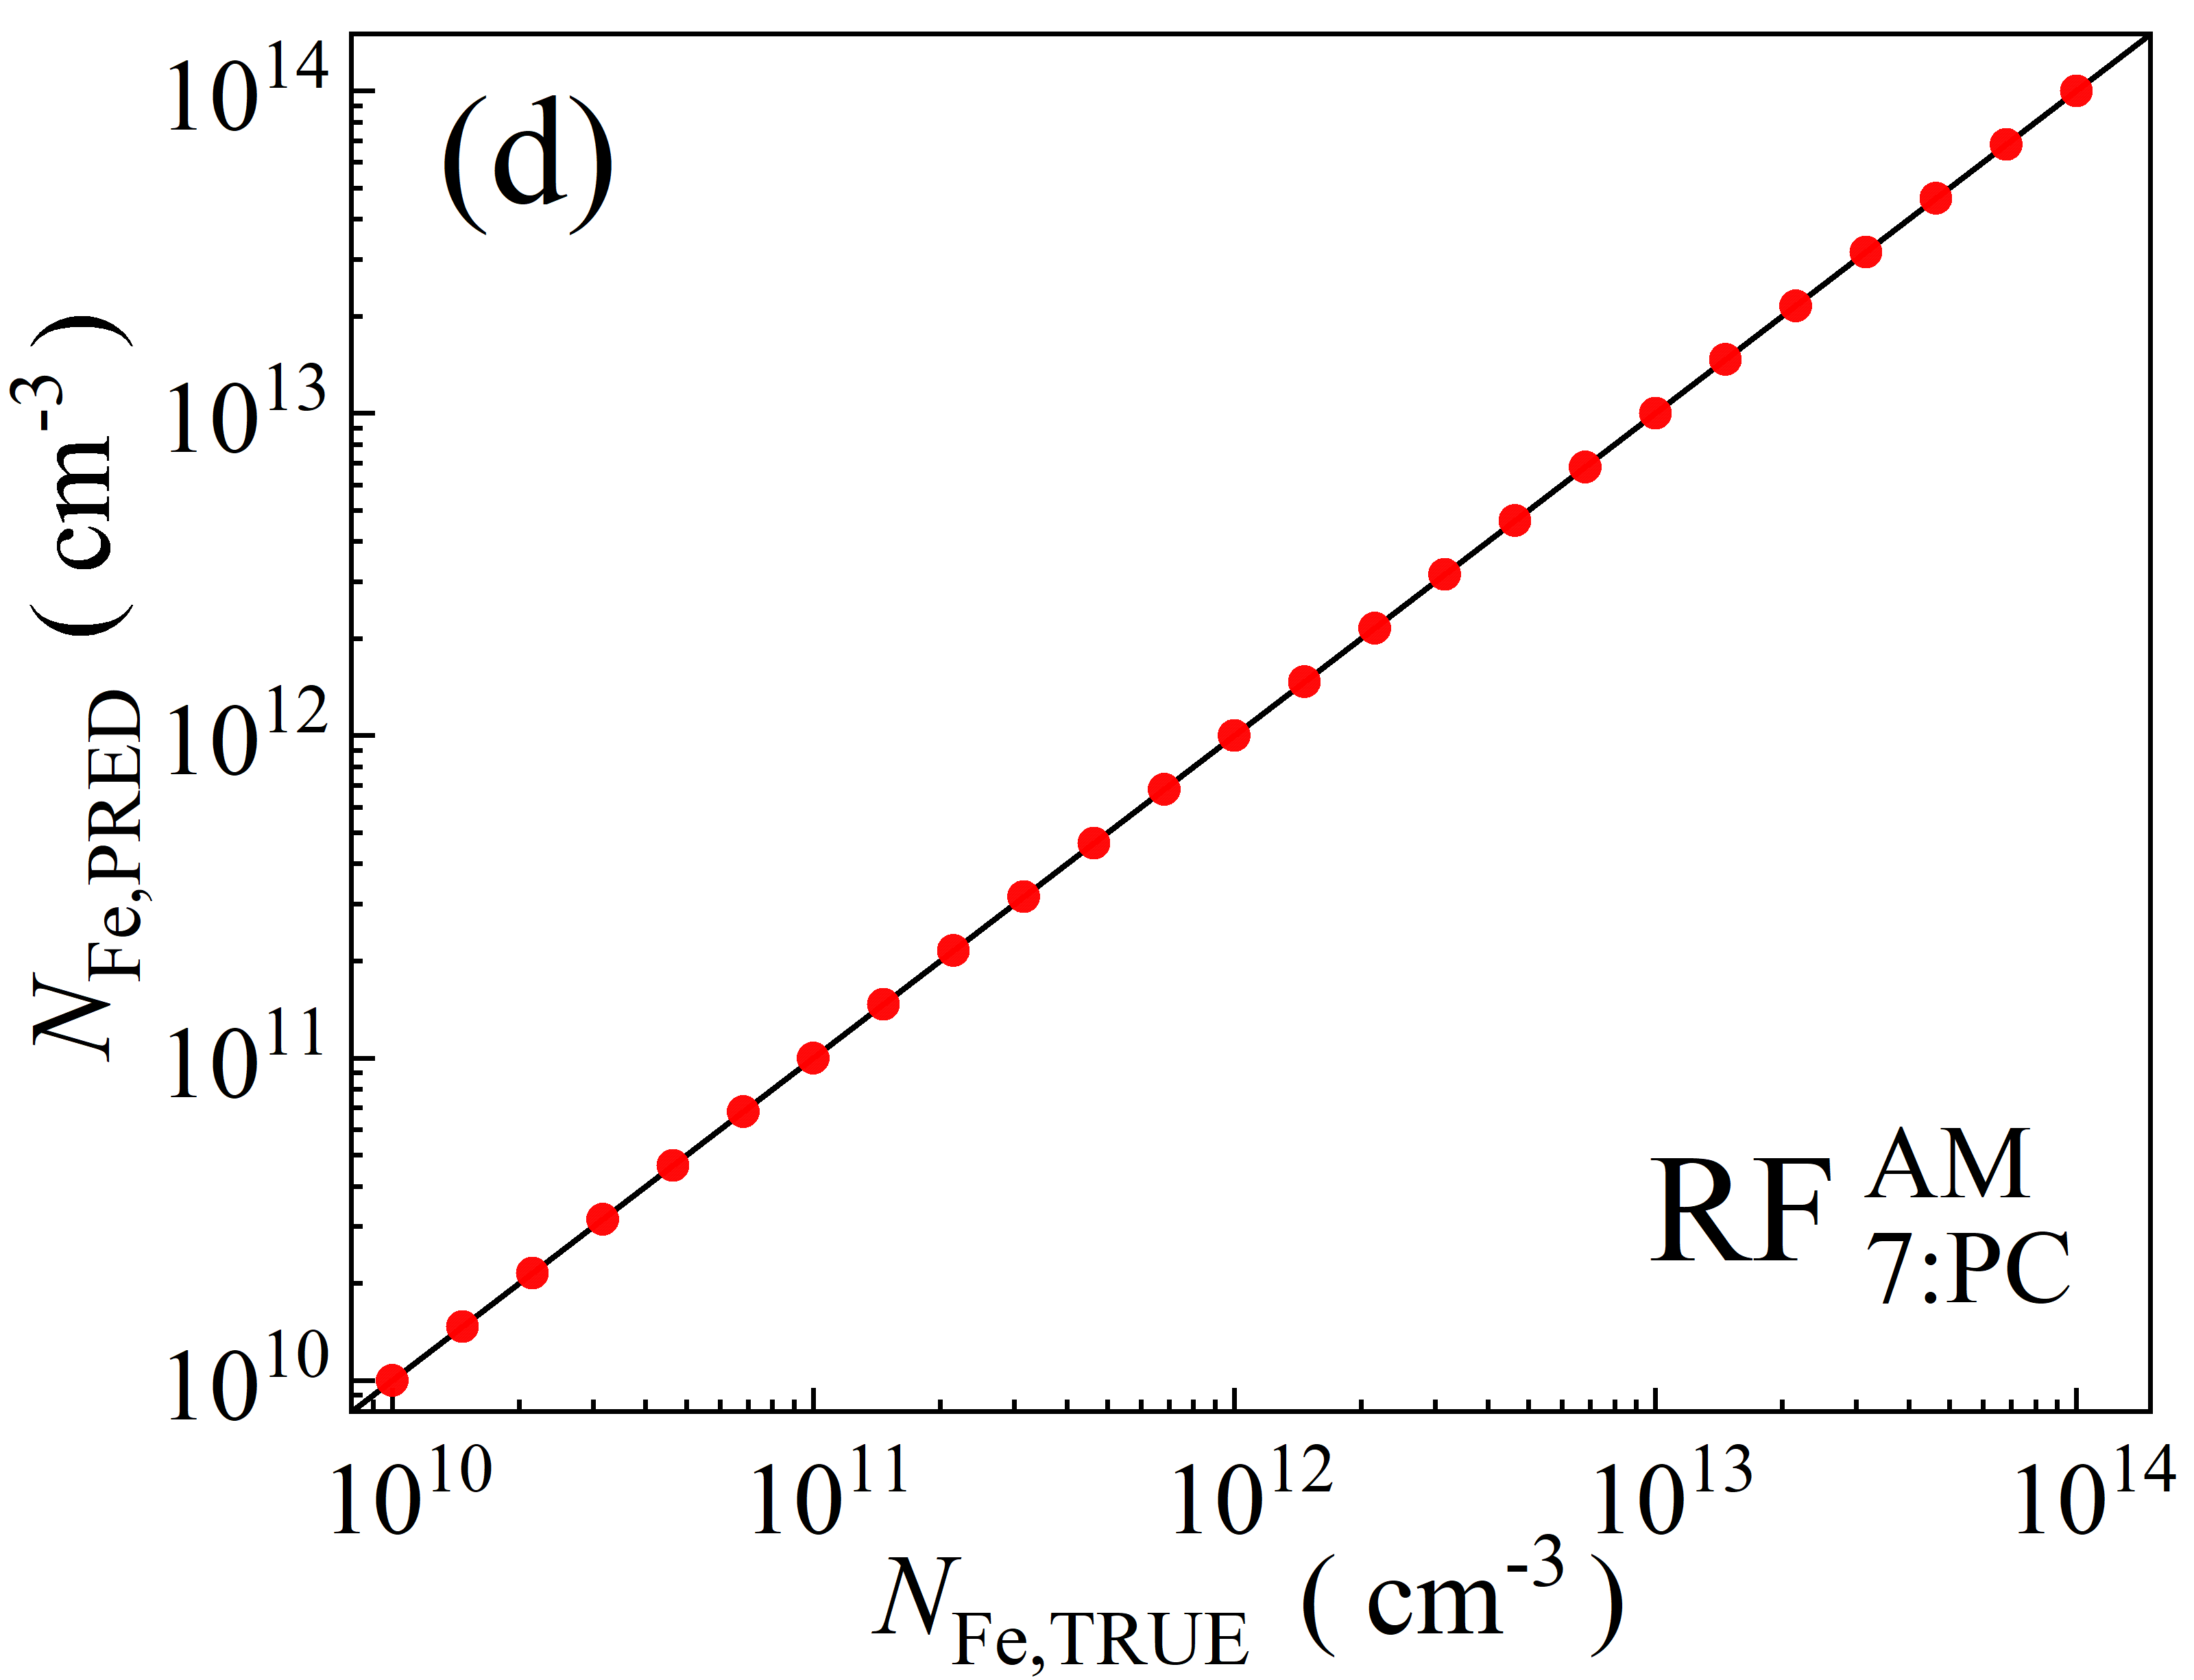
\includegraphics[width=0.4\linewidth]{Fig3d.png}
  \caption{Rise of the dissociated FeB pair concentration under the illumination by sources Orion (a), Osram (b), GE (c) of different intensities ($T=340$~K).
  Panel (d) compares the effect of different light sources.
  The marks are the experimental results, the lines are the fitting by Equation~(\ref{eqNfe0Exp}).
   }
  \label{fig3}
\end{figure}


Considering Equation~(\ref{eqNfeill}), the experimentally obtained dependencies $N_\mathrm{Fe,0}(t_\mathrm{ill})$ were fitted using the function
\begin{equation}
\label{eqNfe0Exp}
N_\mathrm{Fe,0}(t_\mathrm{ill})=A\exp(-t_\mathrm{ill}/\tau_\mathrm{dis})
+B\,,
\end{equation}
where
$\tau_\mathrm{dis}$ is the characteristic dissociation time,
and $B$ means the concentration of dissociated pairs at the saturation.
The fitting parameters are collected in \textbf{Table~\ref{tb1}},
including the coefficient of determination $R^2$.
The high values of $R^2$ (greater than 0.99) confirm the suitability of the chosen fitting formula.

\begin{table}
 \caption{ Fitting parameters of experimental dependencies $N_\mathrm{Fe,0}(t_\mathrm{ill})$
 using Equation~(\ref{eqNfe0Exp}) and defect parameters estimated using Equations~(\ref{eqTauRd}-\ref{eqFefit}).
}
 \label{tb1}
  \begin{tabular}[htbp]{@{}ccccccc@{}}
    \hline
    $W_\mathrm{ill}$~[mW] & Light source & \multicolumn{3}{c}{fitting parameters}&\multicolumn{2}{c}{defect parameters} \\
     &  & $\tau_\mathrm{dis}$ [s] & $B$ [$10^{12}$~cm$^3$] & $R^2$ & $R_d$ [$10^{-3}$~s$^{-1}$] & $N_\mathrm{Fe,tot}$ [$10^{12}$~cm$^{-3}$] \\
    \hline
    750  & Orion  & $2.2\pm0.2$ & $8.6\pm0.1$ & 0.993 &450&8.6\\
    700  & Orion  & $2.7\pm0.2$ & $8.7\pm0.1$ & 0.995 &370&8.7\\
         & Osram  & $2.4\pm0.2$ & $8.6\pm0.1$ & 0.992 &410&8.6\\
    600  & Orion  & $3.7\pm0.2$ & $8.65\pm0.06$ & 0.998&270&8.7 \\
         & Osram  & $3.0\pm0.2$ & $8.69\pm0.08$ & 0.995&330&8.7 \\
    500  & Orion  & $5.5\pm0.2$ & $8.65\pm0.04$ & 0.999&180&8.7 \\
         & Osram  & $4.5\pm0.1$ & $8.7\pm0.1$ & 0.998&220&8.8 \\
    400  & Orion  & $8.8\pm0.3$ & $8.74\pm0.06$ & 0.998&110&8.8 \\
         & Osram  & $6.1\pm0.2$ & $8.63\pm0.08$ & 0.997 &160&8.7\\
         & GE  & $3.6\pm0.3$ & $8.7\pm0.1$ & 0.996 &280&8.7\\
    300  & Orion  & $15.7\pm0.6$ & $8.6\pm0.1$ & 0.998 &62&8.8\\
         & Osram  & $12.4\pm0.1$ & $8.69\pm0.02$ & 0.999&79&8.8 \\
         & GE  & $6.5\pm0.2$ & $8.69\pm0.05$ & 0.998 &150&8.8\\
    200  & Orion  & $35\pm3$ & $8.5\pm0.3$ & 0.998 &27&8.8\\
         & Osram  & $24\pm1$ & $8.6\pm0.1$ & 0.999 &40&8.9\\
         & GE  & $15.1\pm0.5$ & $8.7\pm0.1$ & 0.999 &65&8.8\\
    \hline
  \end{tabular}
\end{table}



One can see from Equations~(\ref{eqNfeill}) and (\ref{eqNfe0Exp}) that
the fitting parameters relate to defect characteristics:
\begin{equation}
\label{eqTauRd}
\tau_\mathrm{dis}^{-1}=R_a+R_d\,,
\end{equation}
\begin{equation}
\label{eqFefit}
B=N_\mathrm{Fe,tot}\frac{R_d}{R_d+R_a}\,.
\end{equation}

The fitting parameters
with considering the association rate of $1.68\times10^{-3}$~s allow us
to calculate the values of $N_\mathrm{Fe,tot}$ and $R_d$, which are also collected in Table~\ref{tb1}.
As seen, the calculated values of the impurity iron atom concentration
$N_\mathrm{Fe,tot}=(8.7\pm0.1)\times10^{12}$~cm$^{-3}$ are expectably independent of the light source and illumination intensity $W_\mathrm{ill}$.
This confirms the accuracy of the analysis.
Contrariwise, the FeB dissociation rate may vary significantly with both the intensity value and the used light source.

According to Wijaranakula \cite{FeB:kinetic}, the concentrations of interstitial iron atoms $N_\mathrm{Fe,eq}$ and FeB pairs
$N_\mathrm{FeB}$ before the illumination at the specified value of $N_\mathrm{Fe,tot}$ and $T=340$~K are $1.3\times10^{12}$~cm$^{-3}$ and $7.4\times10^{12}$~cm$^{-3}$, respectively.
The values of $N_\mathrm{Fe,eq}$ and $N_\mathrm{FeB}$ were used to estimate the minority carrier diffusion length $L_n$
in the base of the used solar cell.
It was assumed that the dominant recombination processes are SRH recombination at Fe$_i$ and FeB and intrinsic recombination.
The required value of electron mobility $\mu_n$ was taken from Klaassen \cite{KLAASSEN953},
the capture cross sections and energy levels for Fe$_i$ and FeB from Rougieux \emph{et al.} \cite{ROUGIEUX2018},
the parameters of band-to-band radiative recombination and Auger recombination from
Niewelt \emph{et al.} \cite{Brad2022} and Black \& Macdonald \cite{AugerSi2022}, respectively.
The calculated value was found to be $L_n=80$~$\mu$m,
which is very close to 86~$\mu$m  obtained from the study of temperature dependencies of short-circuit current, see Supplementary materials.

\subsection{Carrier generation rate estimation}\label{SecG}

The light-induced dissociation rate of FeB pairs is well known
to be dependent on the carrier generation rate (see Eq.~(\ref{eqRd})).
Our next aim was determining the values of $G$ for various light sources.
\textbf{Figure~\ref{fig4}} shows the measured spectral intensity of illumination, $w_\mathrm{ill}$, incident onto the sample surface.
It is crucial to highlight that our focus is specifically on the light reaching the sample;
hence, the brought spectra are distorted not only by the absorption of the lamp reflector and protective glass, but also by absorption in the fiber
utilized to transmit the light flux to the solar cell.
Other researchers have considered similar modifications of the illumination spectra \cite{Libra2017}.
Figure~\ref{fig4}a displays discrepancies in the illumination spectra obtained from different light sources,
attributed to variations in the operational temperatures of the halogen lamps and differences in reflectors
(photos of the lamps are in the inset of Figure~\ref{fig4}a).
It is important to note that the upper limit of the spectra in Fig~\ref{fig4} (1120~nm)
is limited by the silicon bandgap, which, according to Passler \cite{Pasler}, corresponds to 1.11~eV at 340 K.
Furthermore, Figure~\ref{fig4}b demonstrates the change in the Osram spectrum with integral intensity increasing.
Notably, in addition to the expected increase in the curve's area, a minor spectrum shift towards shorter wavelengths is observed.
This behavior is typical for all used light sources.


\begin{figure}
\centering
  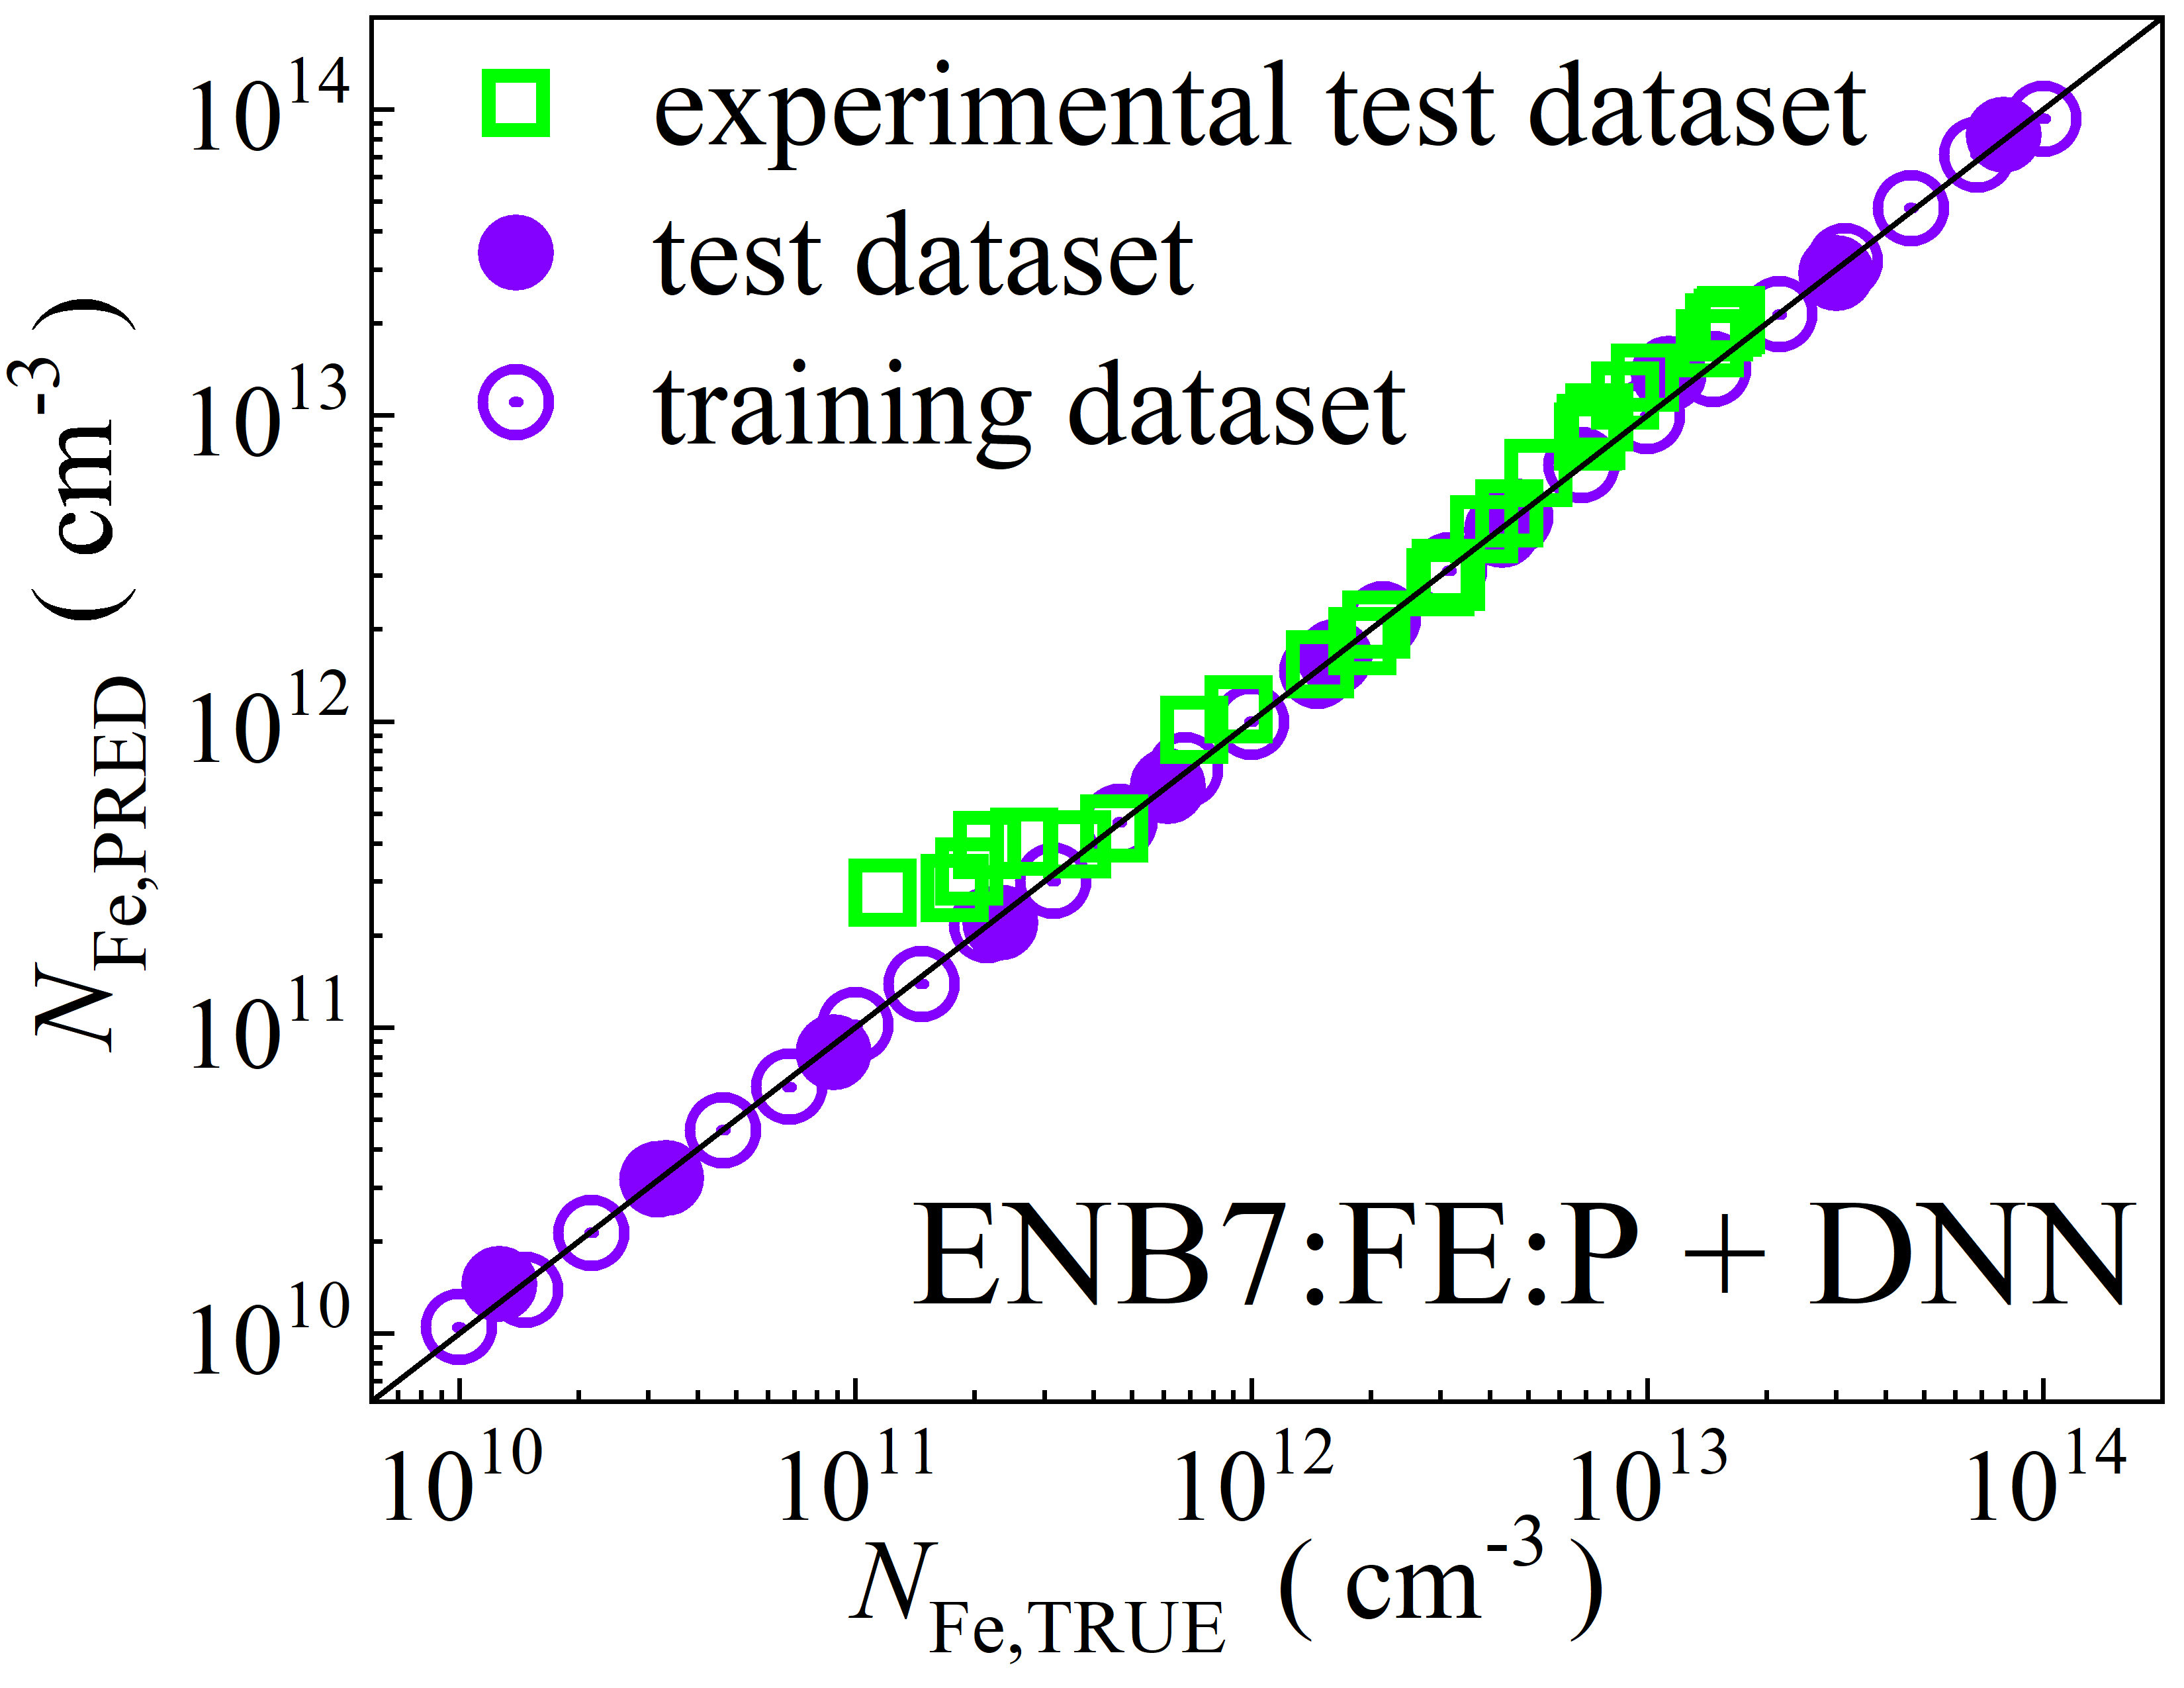
\includegraphics[width=0.4\linewidth]{Fig4a.png}
  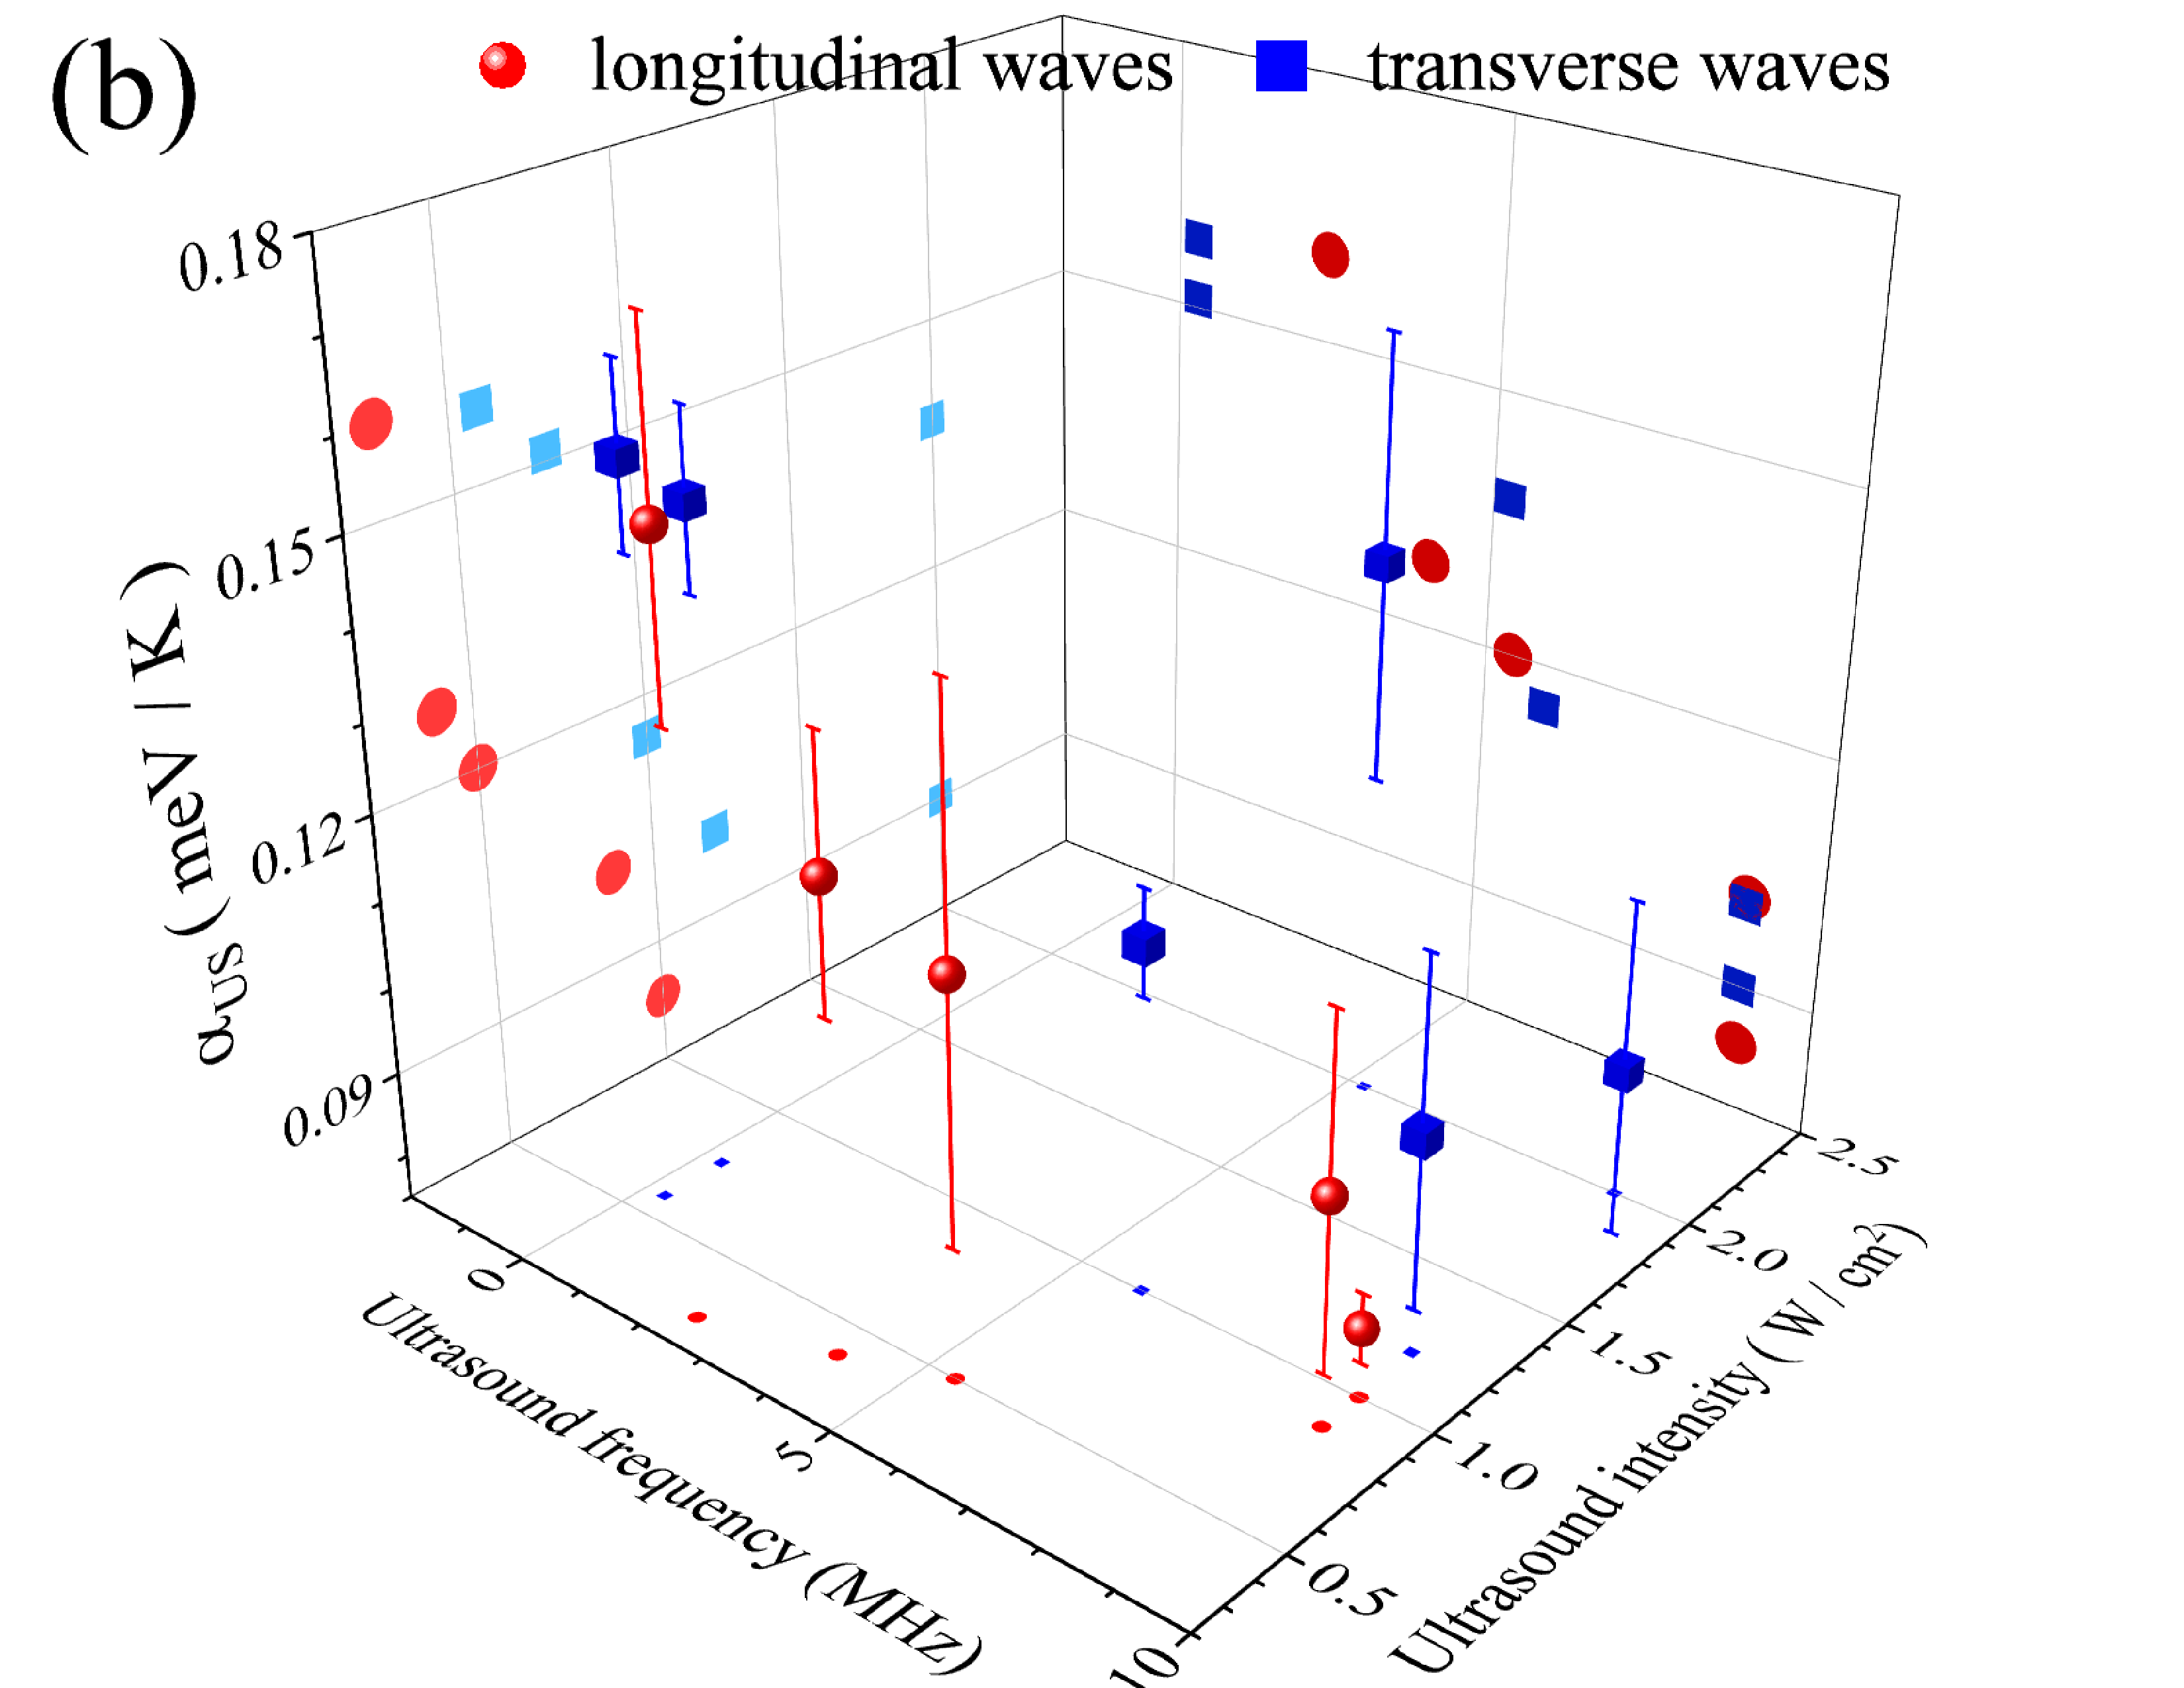
\includegraphics[width=0.4\linewidth]{Fig4b.png}
  \caption{
  The spectra of sample illumination under different light sources with the same integral intensity $W_\mathrm{ill}=400$~mW (a) and Osram source at various $W_\mathrm{ill}$ values (b).
 The inset shows photos of light sources.
}
  \label{fig4}
\end{figure}


The carrier generation rate was estimated as follows:
\begin{equation}
\label{eqGint}
G=\int g(\lambda) d\lambda\,,
\end{equation}
where the spectral density of carrier generation rate
\begin{equation}
\label{eqGspectr}
g=\frac{w_\mathrm{ill}\lambda}{hc}\frac{(1-R)A_\mathrm{bb}}{S\,d_\mathrm{eff}}\,,
\end{equation}
where $n_\mathrm{ph}=\frac{w_\mathrm{ill}\lambda}{hc}$ is the spectral photon flux,
$R$ is the reflectance,
$A_\mathrm{bb}$ is the band-to-band fraction of the absorptance,
$S$ is the illuminated area of the sample,
$d_\mathrm{eff}$ is the effective width of carrier generation.

When calculating the value of $R$, we employed an approach \cite{KostRefl2000},
which considers the presence of antireflective and passivating layers on the front surface of the sample,
as well as the effects of multiple reflections.
The resulting spectral dependence of $R$ is shown in Figure~S3 of the Supplementary materials.

The expression for the e-h pair generating fraction of the Lambertian absorptance in a solar cell
can be written as \cite{Schaefer2018}:
\begin{equation}
\label{eqAbb}
A_\mathrm{bb}(\lambda)=\frac{\alpha_\mathrm{bb}}{\alpha_\mathrm{bb}+\alpha_\mathrm{fca}}\frac{(1-T_r)(1+T_r)n_r^2}{n_r^2-(n_r^2-1)T_r^2}\,,
\end{equation}
with
\begin{eqnarray*}
T_r&=&(1-x)\exp(-x)+x^2E_1(x)\,,\\
x&=&(\alpha_\mathrm{bb}+\alpha_\mathrm{fca})d\,,\\
E_1(x)&=&\int_x^\infty t^{-1}\exp(-t)dt\,,
\end{eqnarray*}
where
$\alpha_\mathrm{bb}$ is the band-to-band absorption coefficient;
$\alpha_\mathrm{fca}$ is the free carrier absorption coefficient;
$n_r$ is the refractive index;
$d$ is the width of the device.

In our calculations of $A_\mathrm{bb}$ by using Equation~(\ref{eqAbb}), we took  $\alpha_\mathrm{bb}$ and
$n_r$ from Green\cite{Green2022}, $\alpha_\mathrm{fca}$  from Baker-Finch \emph{et al.} \cite{SiFCA}.
The spectral dependence of $A_\mathrm{bb}$ can be found in Supplementary materials (Figure~S5).

When determining the carrier generation volume, we applied the Bowden\&Sinton  approach \cite{Bowden2007} to thick silicon wafers,
where the diffusion length or light absorption depth is significantly less than the sample thickness.
In this case, the non-equilibrium carriers are concentrated near the illuminated surface,
making using the arithmetic average of carrier concentration unsuitable.
Therefore, the average values are calculated using carrier concentration as a weighting function,
and effective generation width is determined as follows \cite{Bowden2007}:

\begin{equation}
\label{eqdeff}
d_\mathrm{eff}(\lambda)=\frac{\left(\int_0^d \Delta n dx\right)^2}{\int_0^d \Delta n^2 dx}\,,
\end{equation}
where
$\Delta n$ is the increase in minority carrier density due to illumination
\begin{equation}
\label{eqdeln}
\Delta n (x)=\frac{\alpha_\mathrm{bb} n_\mathrm{ph} L_n^2 q}{(\alpha_\mathrm{bb}^2 L_n^2-1)kT\mu_n}
\left[\exp\left(-\frac{x}{L_n}\right)-\exp\left(-\alpha_\mathrm{bb} x\right)\right]\,.
\end{equation}
In calculations, we used $L_n$ value, determined in Subsection~\ref{SecR}.
Figure~S4 (Supplementary materials) shows some dependencies of $d_\mathrm{eff}(\lambda)$ for different $L_n$ values.

The consideration of dependencies $R(\lambda)$, $A_\mathrm{bb}(\lambda)$, and $d_\mathrm{eff}(\lambda)$ modifies
the spectral density of carrier generation rate compared to the spectrum of incident light,
leading to an increased contribution to e-h pairs generated with shorter wavelengths,
as illustrated in \textbf{Figure~\ref{fig5}a}.
In \textbf{Figure~\ref{fig5}b}, variations of the total carrier generation rate $G$ with increasing light intensity for different light sources are plotted.
It is evident that differences exist between the light sources at the same $W_\mathrm{ill}$,
however, they are within 2 percent of the values;
Orion source reveals the highest carrier generation rates.

\begin{figure}
\centering
  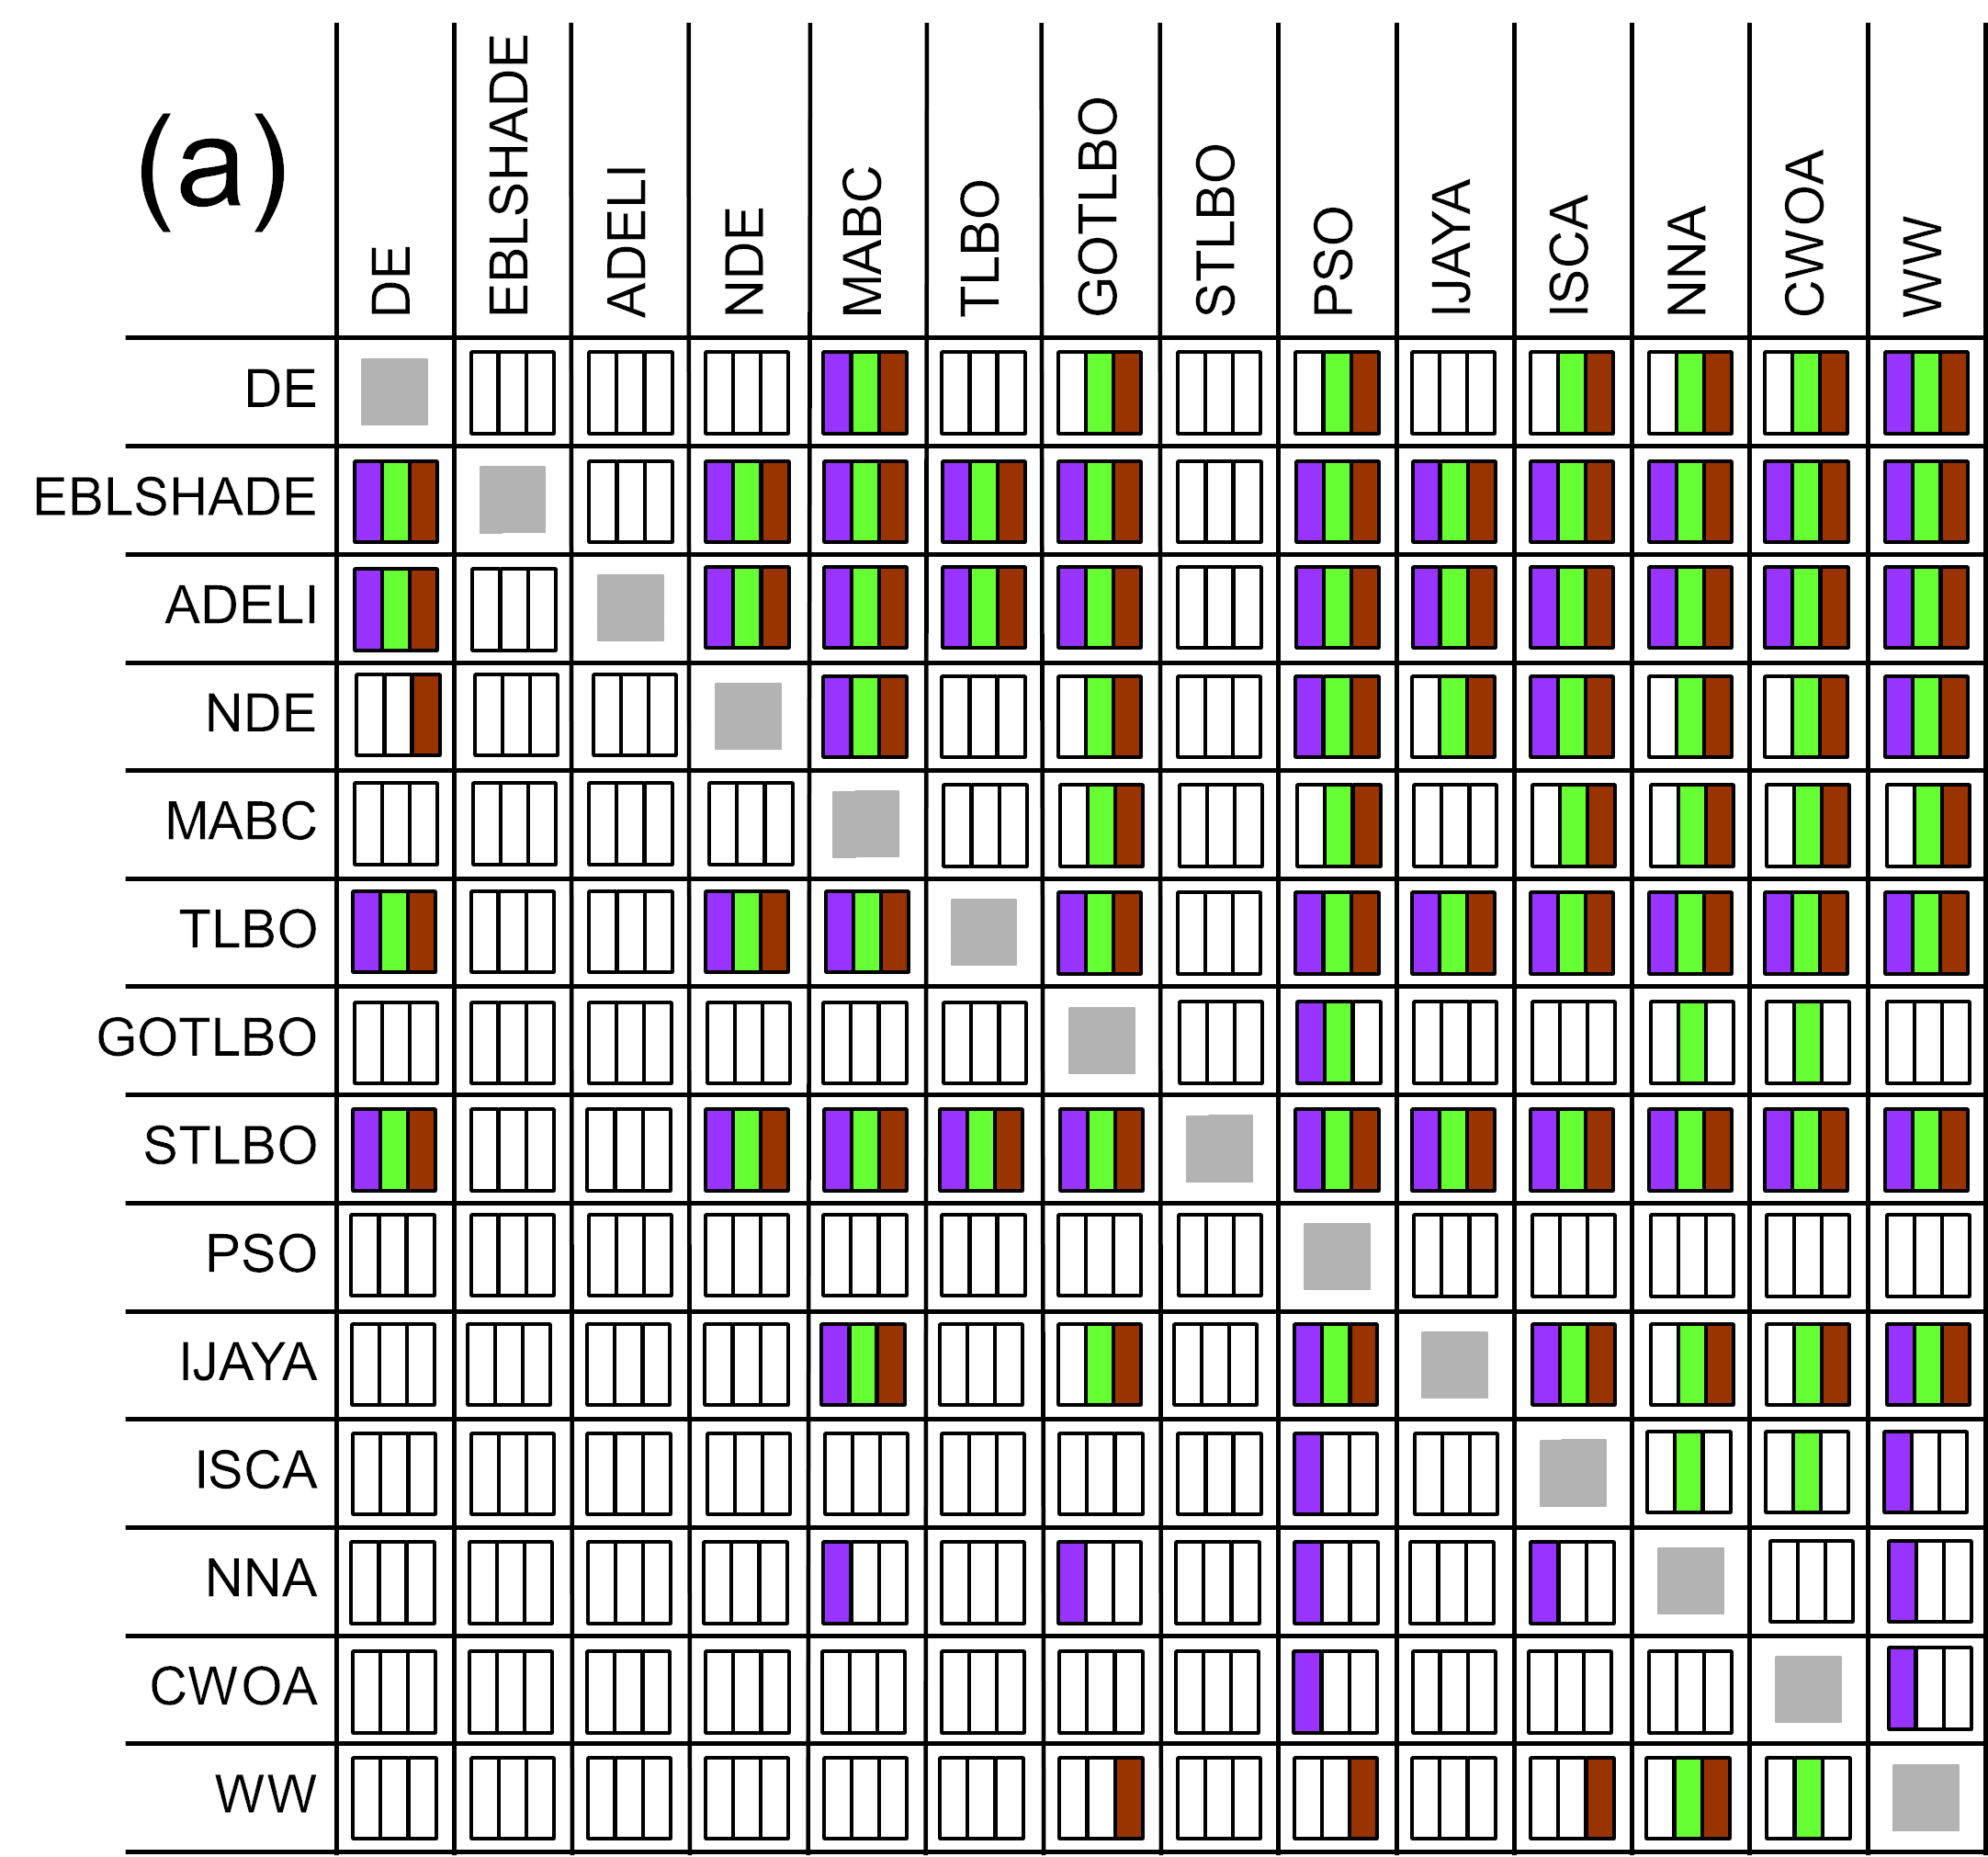
\includegraphics[width=0.4\linewidth]{Fig5a.png}
  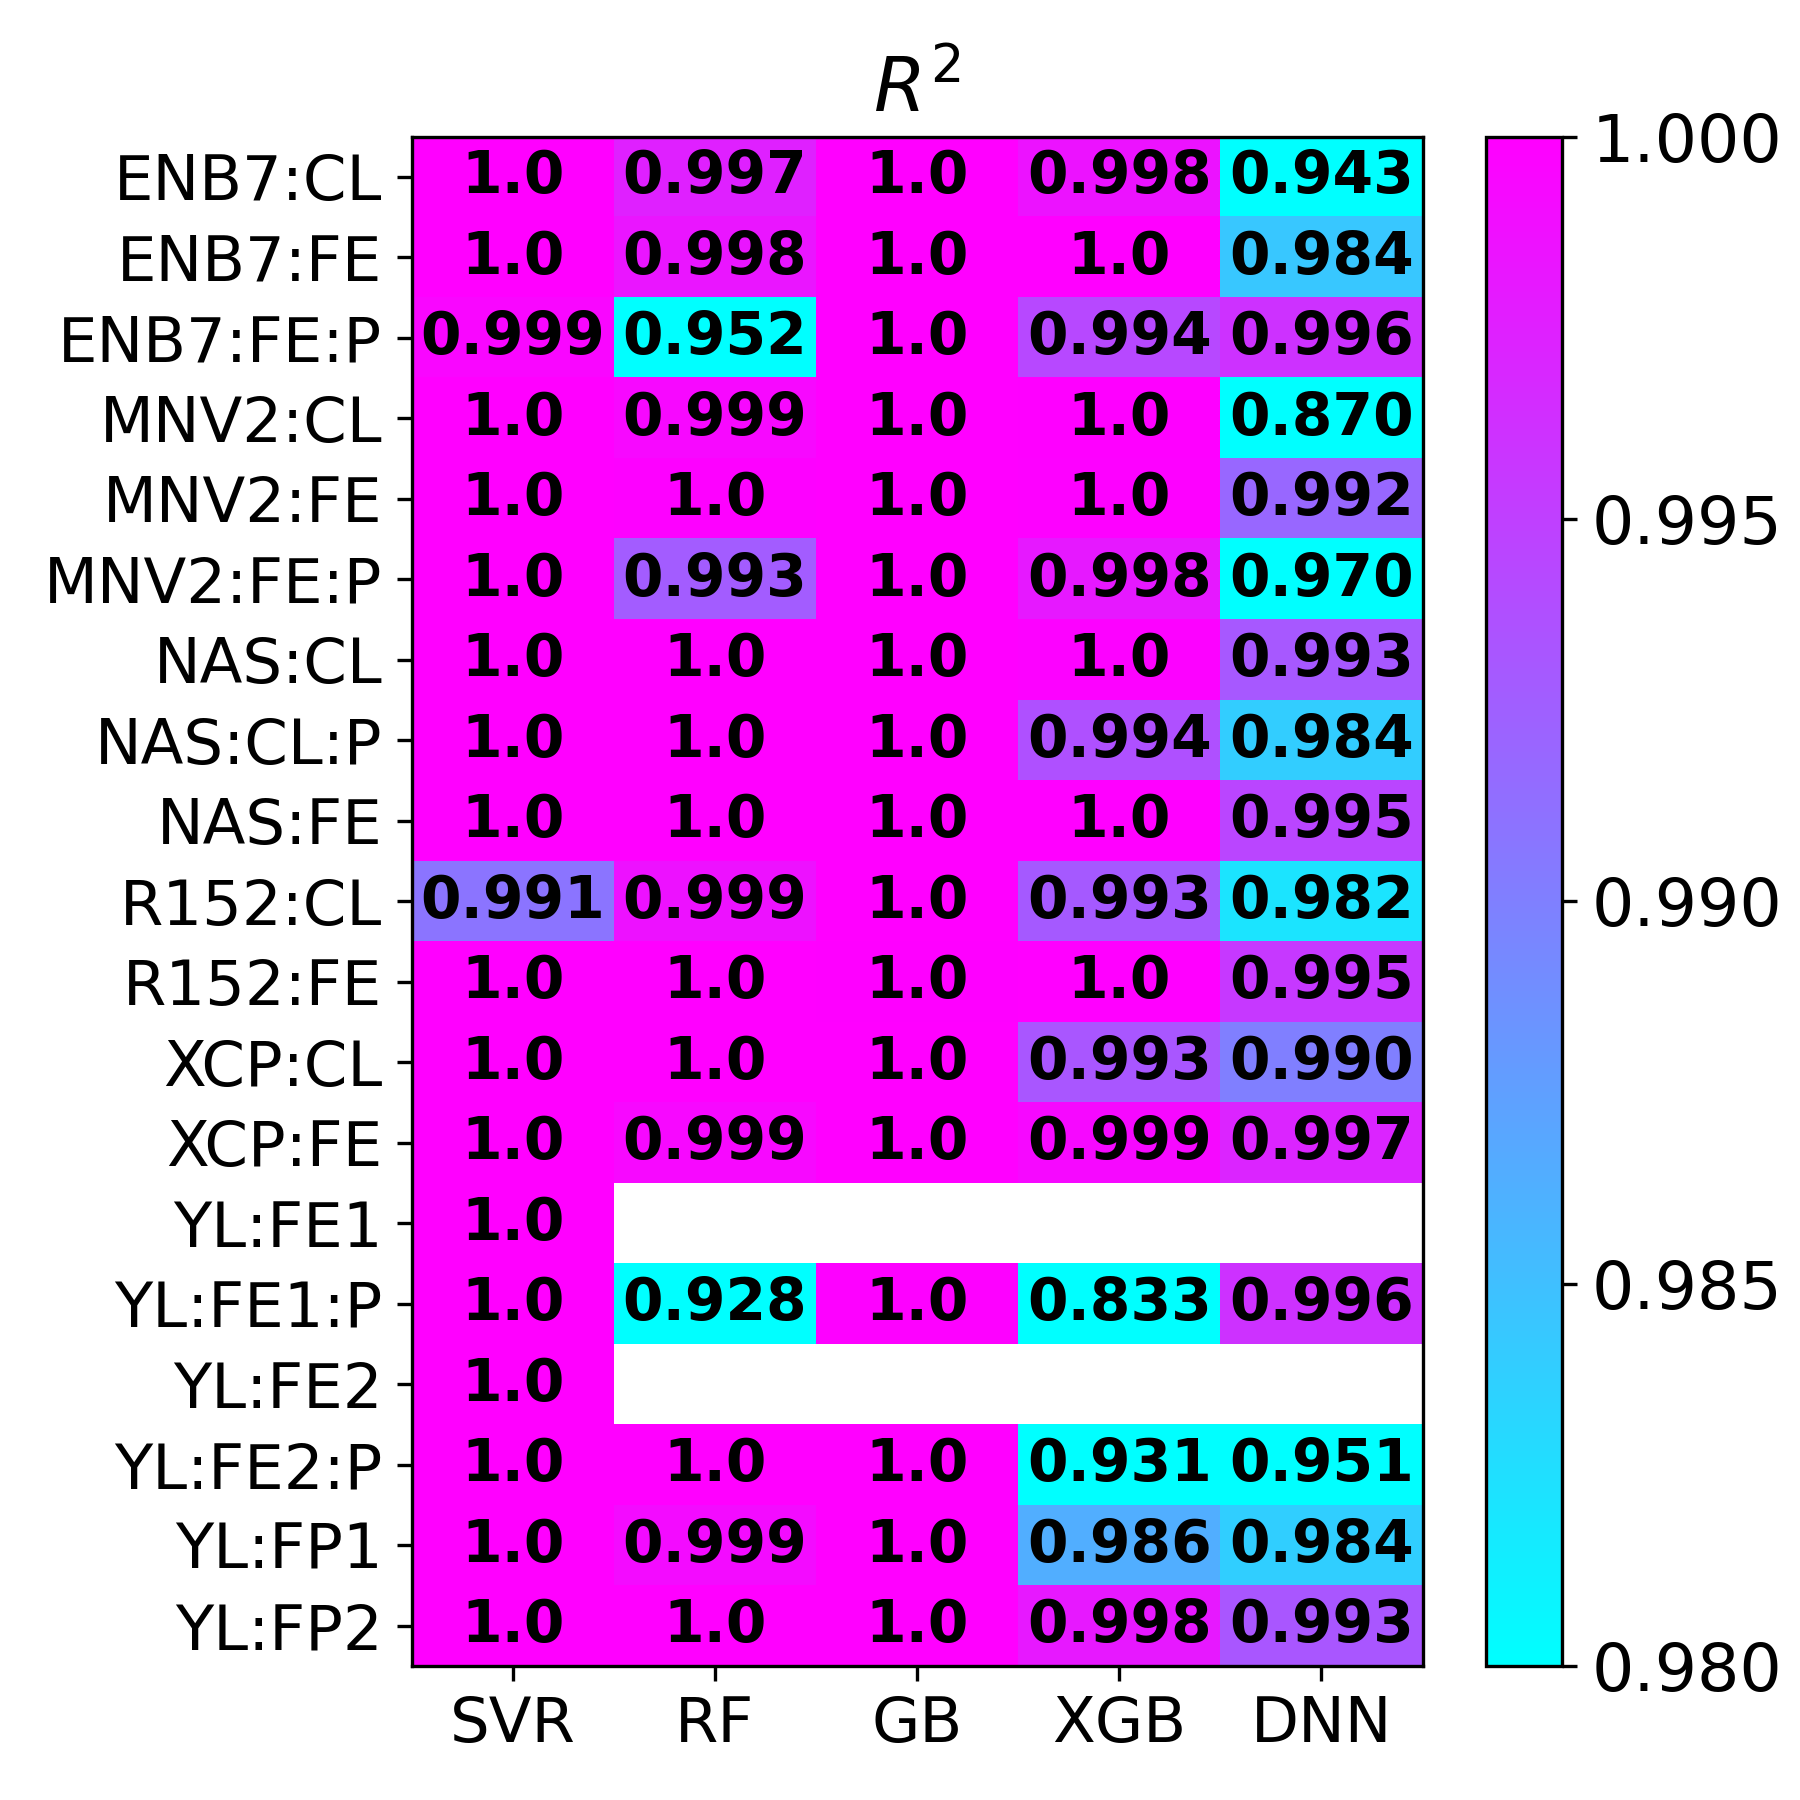
\includegraphics[width=0.4\linewidth]{Fig5b.png}
  \caption{
  (a) Spectral densities of photon flux from Orion source at $W_\mathrm{ill}=400$~mW (left axis, solid line) and carrier generation rate (right axis, dashed line).
  (b) Dependencies of carrier generation rate on illumination intensity for different light sources.
  }
  \label{fig5}
\end{figure}

Thus, the discrepancies noticed previously in the value of $R_d$ (see Table~\ref{tb1}) under identical illumination intensity levels
cannot be attributed to variations in the carrier generation rate among different light sources,
even when considering the quadratic dependency (\ref{eqRd}) of the dissociation rate on $G$.
Hence, there must be another underlying cause for these differences.


\subsection{Effect of illumination spectrum on FeB pair decay}\label{SecLast}

The dependencies $R_d (G)$ in the logarithmic scale are presented in \textbf{Figure~\ref{fig6}a}.
The lines are quadratic dependencies $\propto G^2$ fitting the experimental data using Equation~(\ref{eqRd}).
High correlation coefficients exceeding 0.998 validate the applicability of the quadratic dependence.
It should be noted that Khelifati \emph{et al.} \cite{FeBKin2019} stipulated the change of $R_d$ to
$R_d\left(1+\tau_\mathrm{FeB}/\tau_\mathrm{other}\right)^2$ ($\tau_\mathrm{FeB}$ is the lifetime associated with recombination on FeB pairs)
on the left side of Equation~(\ref{eqRd}).
However, in our case $\tau_\mathrm{other}\gg \tau_\mathrm{FeB}$, as mentioned in Subsection~\ref{SecR}, therefore,
this additional multiplier may be neglected.


\begin{figure}
\centering
  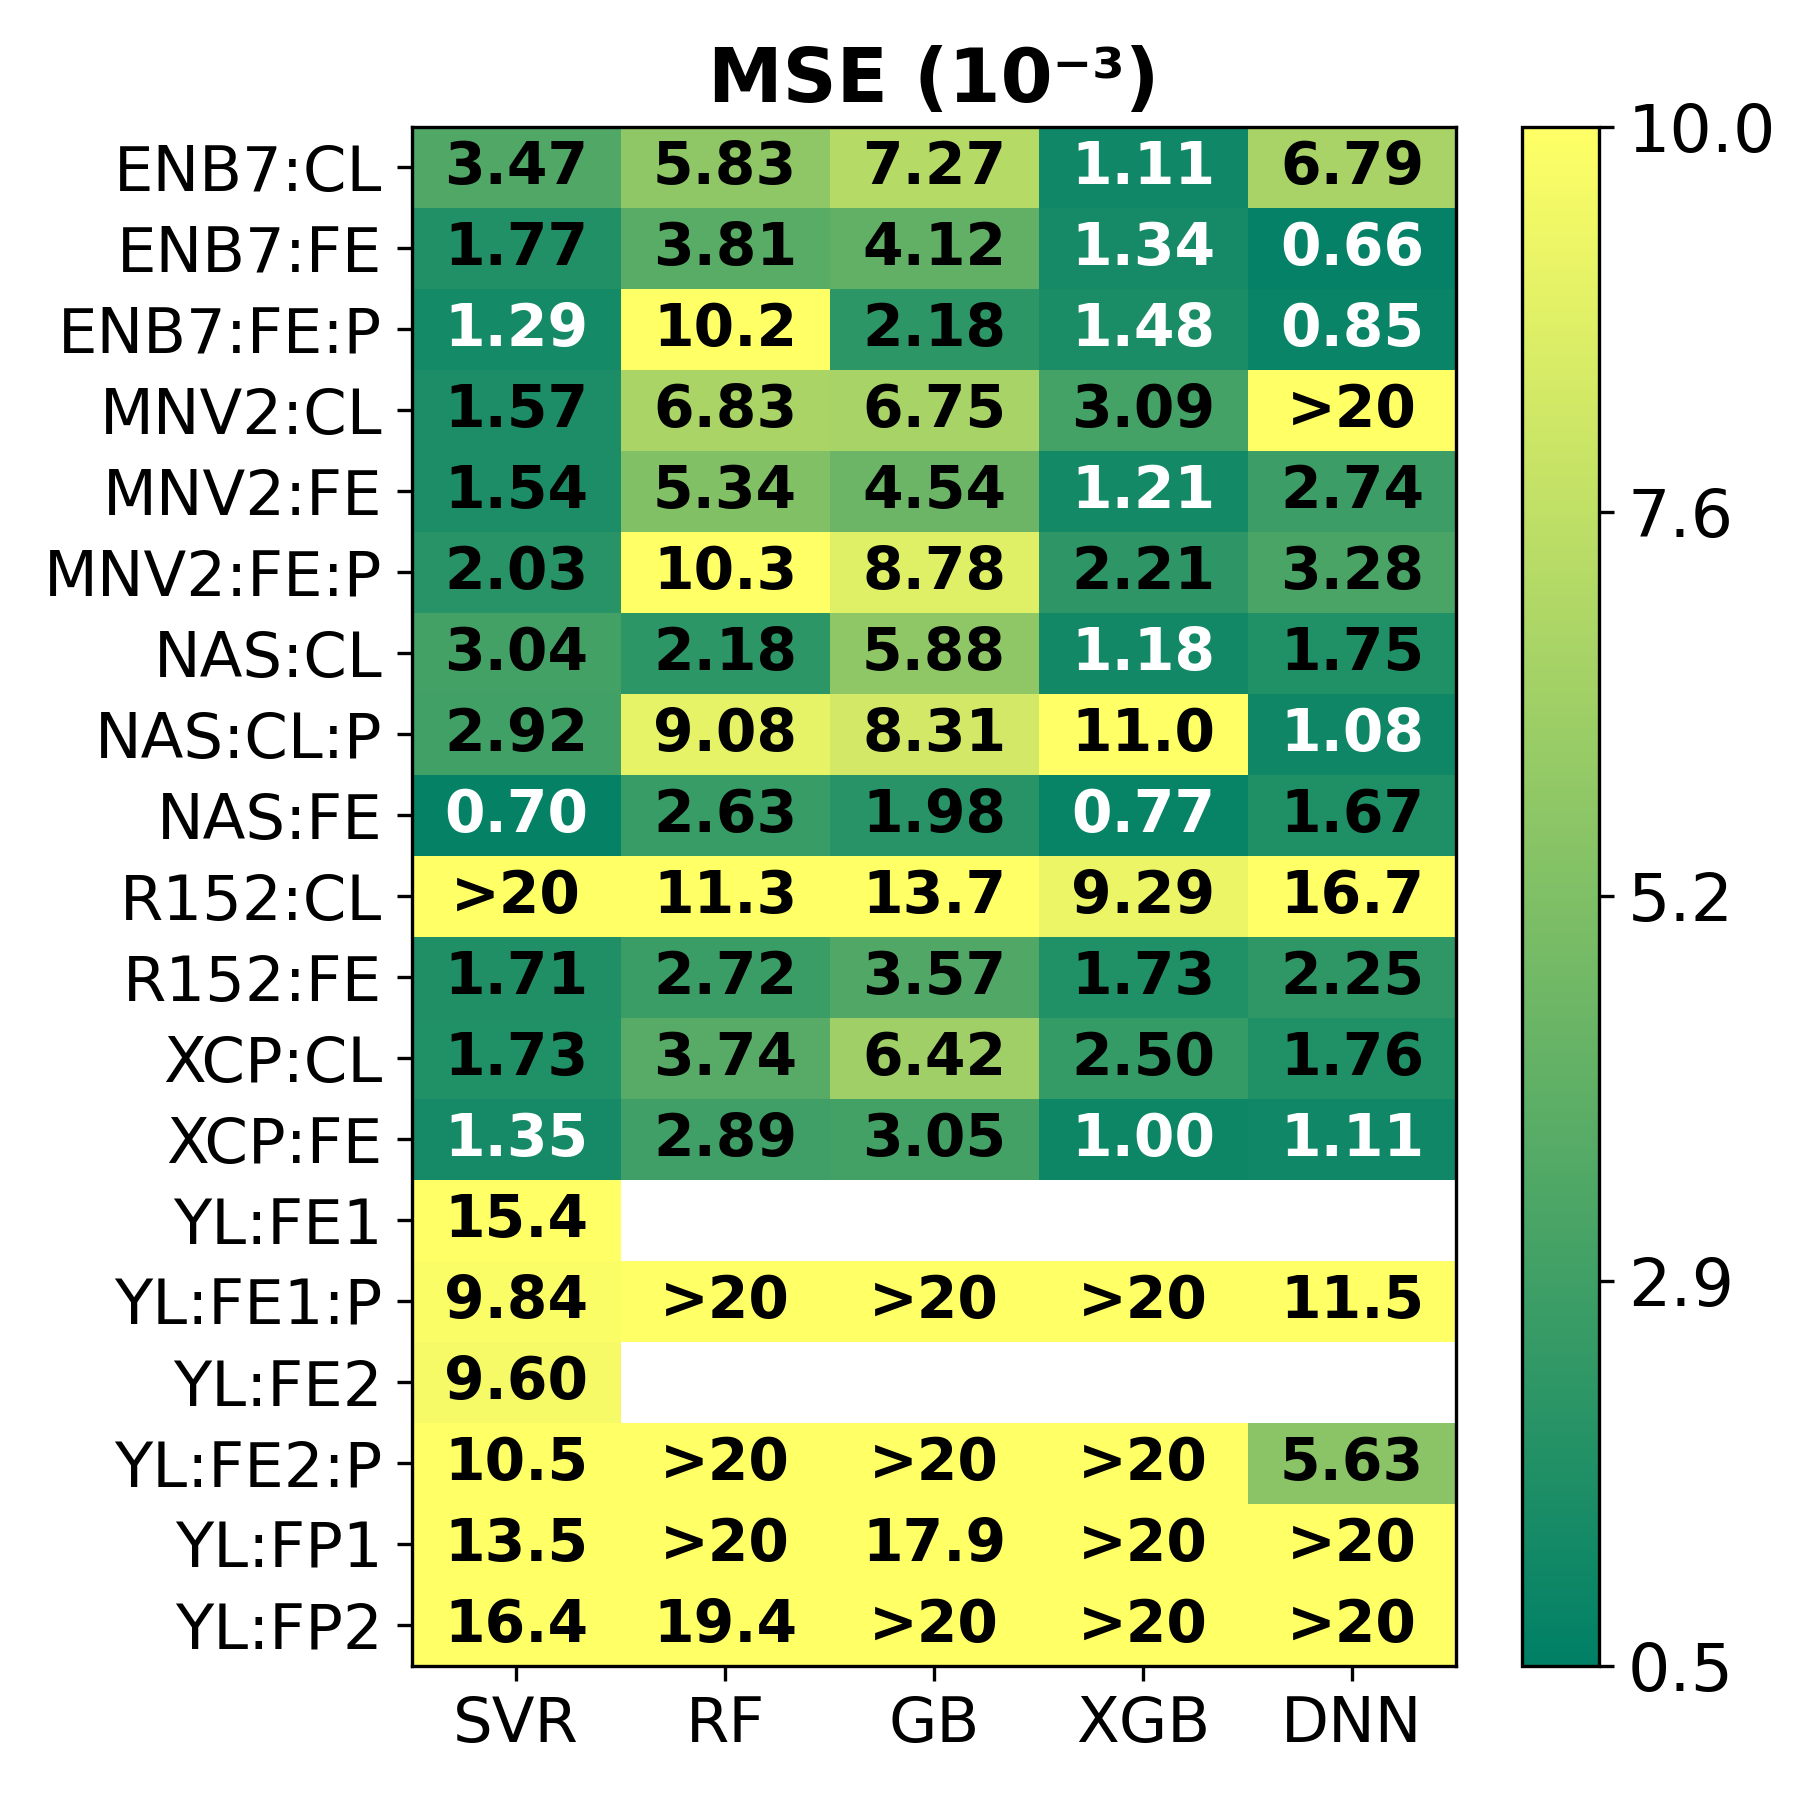
\includegraphics[width=0.4\linewidth]{Fig6a.png}
  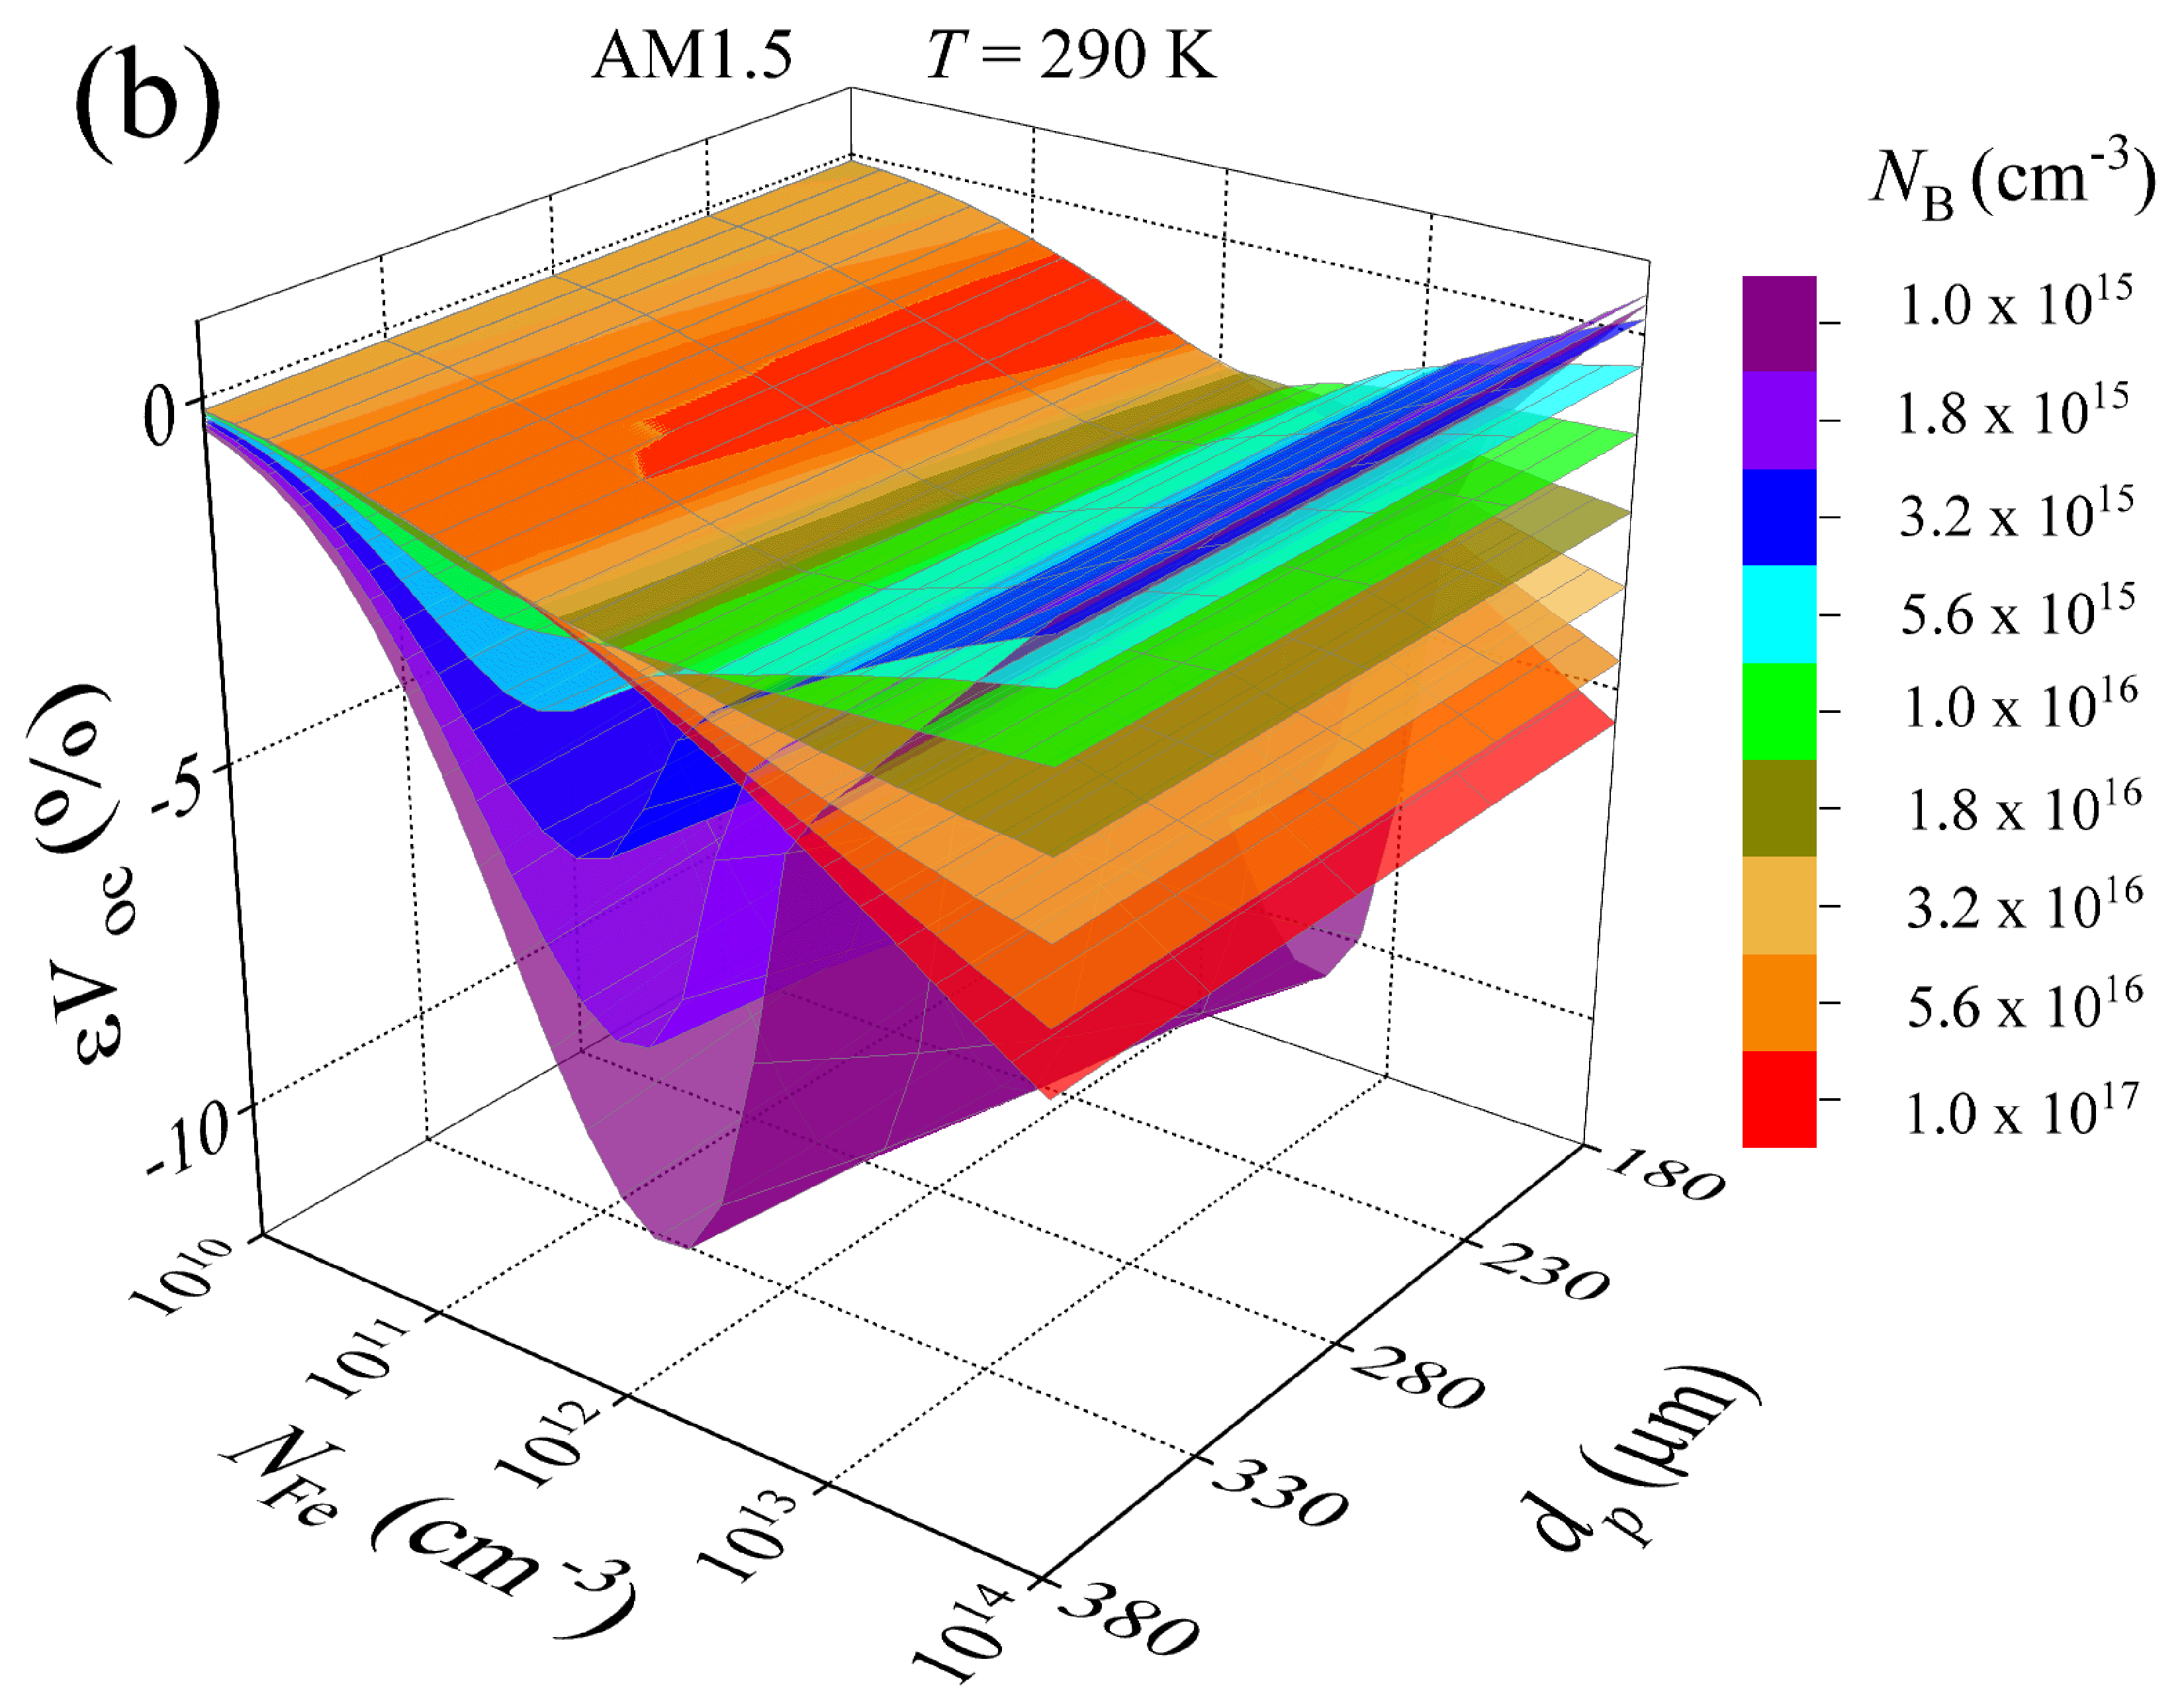
\includegraphics[width=0.4\linewidth]{Fig6b.png}
  \caption{
  (a) FeB pair dissociation rate plotted as $\left(R_d\cdot N_\mathrm{FeB}^2\right)$ versus the light-induced
  generation rate. The solid lines are the fitting with functions $\propto G^2$.
  (b) Dependencies of average photon energy on illumination intensity for different light sources.
  The inset shows pre--factor $K$ vs average photon energy for the different light sources and illumination intensities.
  The lines are linear fitting curves. Coefficients of correlation are shown as well.
  }
  \label{fig6}
\end{figure}

The prefactor $K$ values determined from the fitting are
$3.8\times10^{-15}$~s for the GE light source,
$2.0\times10^{-15}$~s for the Osram, and
$1.5\times10^{-15}$~s for the Orion source.
$K$ is an important parameter related to the phenomenon of FeB pair dissociation caused by illumination \cite{FeBKin2019},
and the values obtained in this study are comparable to those ($4.2\times10^{-17}-5\times10^{-15}$~s) presented in other studies \cite{FeBLight2,FeBAssJAP2014,FeBKin2019}.
It is worth noting that the variety of the constant $K$ values for diverse samples in prior research was attributed
to variations in defect composition and the presence of alternative recombination channels apart from iron--related defects \cite{FeBLight2,FeBAssJAP2014}.
It should be noted that $R_d$ is known to be temperature--dependent \cite{Lagowskii1993}.
However, our values of $K$ were obtained for the same structure under identical conditions, including temperature and integrated light intensity.

So, the obtained data indicate that, when analyzing light--induced dissociation of FeB pairs,
it is necessary to consider not only the quantity of photo--generated charge carriers,
but also the energies of the photons that lead to their appearance.
For such an energy characterization of light sources, we used the average photon energy $<E_\mathrm{ph}>$:
\begin{equation}
\label{eqEaver}
<E_\mathrm{ph}>=\frac{\int \frac{hc}{\lambda}n_\mathrm{ph}(\lambda)d\lambda}{\int n_\mathrm{ph}(\lambda)d\lambda}\,.
\end{equation}


The summary of the results concerning the $<E_\mathrm{ph}>$ values is shown in \textbf{Figure~\ref{fig6}b}.
In particular, it demonstrates a shift of the emission spectrum of light sources
towards shorter waves with an increase in the $W_\mathrm{ill}$ value, as illustrated in Figure~\ref{fig4}b.
Comparing the data in Figure~\ref{fig3}, \ref{fig5}b, \ref{fig6}a, \ref{fig6}b, and Table~\ref{tb1}, one can conclude that
the light--induced dissociation of FeB pairs becomes more pronounced with rising average photon energy.
Specifically, the constant $K$ and the dissociation rate $R_d$ increase and, therefore, the illumination time necessary for a complete complex decay decreases.
Hence, for the dissociation of FeB pairs, the energy expended during the thermalization of non--equilibrium carriers also holds significance.

The obtained results offer some conclusions about the mechanism of FeB dissociation.
As discussed in the literature and previously mentioned, two possible ways of the second decay stage
are typically considered: recharge of the iron ion and REDR.
The latter arises from strong electron--lattice coupling at the defect site and involves utilizing local vibrational energy to promote pair dissociation
\cite{FeBAssJAP2014,Sun2021,Macdonald2004}.
The observed correlation between dissociation rate and photon energy in this study confirms the REDR process.
Specifically, as photon energy increases, the production of non--equilibrium phonons during thermalization also rises.
Furthermore, the increase in $R_d$ value found in the experiment means an active involvement of these quasi--particles in the dissociation of FeB pairs.
Notably, recent research \cite{Sun2021} focusing on a detailed analysis of the dissociation and association reactions of the iron--boron pairs similarly concluded the predominant role of REDR processes.



\section{Conclusion}\label{SecConsl}

The effect of illumination spectra on the dissociation of
FeB pairs in p--Si was investigated.
We reported the results of an experimental study of FeB dissociation rate in a solar cell based on Cz--Si,
which was carried out using different light sources and illumination intensities.


It was shown that the time required for the total dissociation of FeB pairs
not only becomes shorter with increasing the illumination intensity, but also significantly depends
on a light source.
As a result, the determined value of material constant $K$  varies within
$(1.5-3.8)\times10^{-15}$~s
for the used light sources.
The study of the illumination spectra allowed to conclude that the efficiency of FeB photo-dissociation increases with the photon energy.
This, in turn, indicates that
the REDR effect is the dominant factor during the second stage of light--induced dissociation of the FeB pairs.
Furthermore, the obtained results could help to develop defect engineering procedures
for effectively converting unintentional iron impurities in silicon into high--mobility states,
which could significantly impact semiconductor technology.


\section{Experimental Section}
\label{SecExp}

The $n^+$-$p$-$p^+$-Si samples were used in the experiment.
The structure was fabricated from a 380~$\mu$m thick $p$-type boron-doped
Czochralski silicon (100) wafer with hole concentration $p=1.36\times10^{15}$~cm$^{-3}$.
The $n^+$ emitter with a sheet resistance of about $20-30$~$\Omega/\Box$
and  thickness of $0.7$~$\mu$m was formed by phosphorus diffusion.
The anti-recombination isotype barrier was created by using a $p^+$
layer ($10-20$~$\Omega/\Box$, $0.6$~$\mu$m) formed by boron diffusion.
On the front surface, SiO$_2$ (40~nm) and Si$_3$N$_4$ (30~nm) films were formed as antireflective and passivating layers, respectively.
The solid and grid Al contacts were formed by magnetron sputtering on the back and front surfaces, respectively.

A sufficiently high concentration of iron in the examined samples resulted from using impure chemicals during the chemical treatments in the technological process.
This production flaw, which was subsequently corrected, allowed for the creation of model samples to study the effects associated with iron-boron pairs in silicon solar cells.
Details regarding the iron contamination in the sample are described elsewhere \cite{Olikh2021JAP}.

The area of the samples used in the study was $1\times1$~cm$^2$.
The entire surface of the solar cell was illuminated during the experiments.

Three powerful halogen lamps from different manufacturers were used for sample illumination and were employed for the light--induced dissociation of FeB pairs:
\begin{itemize}
  \item Orion Haltlichtspiegel 52240.0, 24 V, 200 W (labeled as ‘‘Orion’’ in the paper);
  \item Osram 64653 HLX ELC, 24 V, 250 W (Osram);
  \item General Electric 43537 H271, 20 V, 150 W (GE);
\end{itemize}
The light sources were powered by the DC Power Supply ITECH IT6332B,
which allowed the current to be set through the lamp with an accuracy of 1~mA.

The illumination was transmitted from the sources to the sample via a fiber.
The source emission at the fiber output underwent a calibration using an optical power and energy meter Thorlabs PM100D and a high-resolution sensor S401C,
thereby enabling a direct assessment of the light flux incident on the sample.
The illumination spectra at the fiber output were recorded using a spectrometer IKC--6 with a germanium photodiode with calibrated spectral sensitivity.

The current-voltage characteristics were measured using a Keithley 2450 source meter and
low--intensity monochromatic light source (light--emitting diode SN--HPIR940nm--1W with light wavelength 940~nm and intensity of about 400~$\mu$W).
The LED radiation intensity was stabilized by a W1209 thermostat and a power supply regulated by a circuit incorporating positive feedback and digital control.

The measurements were carried out at the temperature of 340~K.
The sample temperature was driven by a thermoelectric cooler
controlled byan STS-21 sensor
and maintained constant by a PID algorithm embedded in the software that serves the experimental setup.


\medskip
\textbf{Supporting Information} \par %Please delete the Suppporting Information statement if it is not applicable. Please supply Supporting Information in another file. Supporting information should not be provided in .tex format
Supporting Information is available from the Wiley Online Library or from the author.



% Acknowledgements
\medskip
\textbf{Acknowledgements} \par %delete if not applicable))
The authors are grateful to Prof.~Vitaliy Kostylyov for his help in calculating the reflectance of solar cells.

\medskip
\textbf{Conflict of Interest}\par
The authors declare no conflict of interest.

\medskip
\textbf{Data Availability Statement}\par
The data that support the findings of this study are available from the corresponding author upon reasonable request.
% References
\medskip


\bibliographystyle{MSP}
\bibliography{olikh}


%% Table of contents entry should be 50 - 60 words long
%% Image should be 55 mm broad and 50 mm high or 110 mm broad and 20 mm high
%
%
\begin{figure}
\textbf{Table of Contents}\\
\medskip
  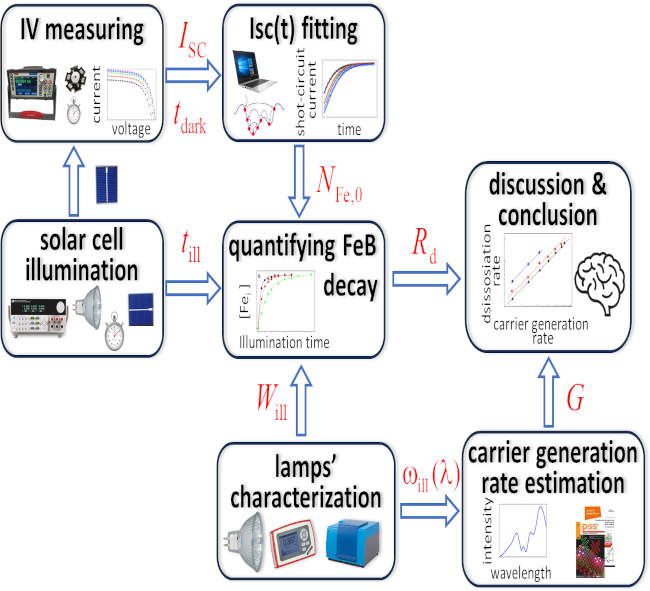
\includegraphics{toc-image.png}
  \medskip
  \caption*{The results of a study on the kinetics of FeB pair dissociation in Cz--Si:B using different light sources are reported. 
  The dissociation rate was shown to depend not only on the intensity but also on the illumination spectrum. 
  The investigation revealed an increase in dissociation efficiency with a decrease in wavelength and highlighted the dominant role of the recombination--enhanced defect reaction.
}
\end{figure}



\end{document}
